%% bare_jrnl_compsoc.tex
%% V1.4b
%% 2015/08/26
%% by Michael Shell
%% See:
%% http://www.michaelshell.org/
%% for current contact information.
%%
%% This is a skeleton file demonstrating the use of IEEEtran.cls
%% (requires IEEEtran.cls version 1.8b or later) with an IEEE
%% Computer Society journal paper.
%%
%% Support sites:
%% http://www.michaelshell.org/tex/ieeetran/
%% http://www.ctan.org/pkg/ieeetran
%% and
%% http://www.ieee.org/

%%*************************************************************************
%% Legal Notice:
%% This code is offered as-is without any warranty either expressed or
%% implied; without even the implied warranty of MERCHANTABILITY or
%% FITNESS FOR A PARTICULAR PURPOSE! 
%% User assumes all risk.
%% In no event shall the IEEE or any contributor to this code be liable for
%% any damages or losses, including, but not limited to, incidental,
%% consequential, or any other damages, resulting from the use or misuse
%% of any information contained here.
%%
%% All comments are the opinions of their respective authors and are not
%% necessarily endorsed by the IEEE.
%%
%% This work is distributed under the LaTeX Project Public License (LPPL)
%% ( http://www.latex-project.org/ ) version 1.3, and may be freely used,
%% distributed and modified. A copy of the LPPL, version 1.3, is included
%% in the base LaTeX documentation of all distributions of LaTeX released
%% 2003/12/01 or later.
%% Retain all contribution notices and credits.
%% ** Modified files should be clearly indicated as such, including  **
%% ** renaming them and changing author support contact information. **
%%*************************************************************************


% *** Authors should verify (and, if needed, correct) their LaTeX system  ***
% *** with the testflow diagnostic prior to trusting their LaTeX platform ***
% *** with production work. The IEEE's font choices and paper sizes can   ***
% *** trigger bugs that do not appear when using other class files.       ***                          ***
% The testflow support page is at:
% http://www.michaelshell.org/tex/testflow/


\documentclass[10pt,journal,compsoc]{IEEEtran}
\usepackage{hyperref}
\usepackage[utf8]{inputenc}
\usepackage [autostyle, english = american]{csquotes}
\MakeOuterQuote{"}

%
% If IEEEtran.cls has not been installed into the LaTeX system files,
% manually specify the path to it like:
% \documentclass[10pt,journal,compsoc]{../sty/IEEEtran}





% Some very useful LaTeX packages include:
% (uncomment the ones you want to load)


% *** MISC UTILITY PACKAGES ***
%
%\usepackage{ifpdf}
% Heiko Oberdiek's ifpdf.sty is very useful if you need conditional
% compilation based on whether the output is pdf or dvi.
% usage:
% \ifpdf
%   % pdf code
% \else
%   % dvi code
% \fi
% The latest version of ifpdf.sty can be obtained from:
% http://www.ctan.org/pkg/ifpdf
% Also, note that IEEEtran.cls V1.7 and later provides a builtin
% \ifCLASSINFOpdf conditional that works the same way.
% When switching from latex to pdflatex and vice-versa, the compiler may
% have to be run twice to clear warning/error messages.






% *** CITATION PACKAGES ***
%
\ifCLASSOPTIONcompsoc
  % IEEE Computer Society needs nocompress option
  % requires cite.sty v4.0 or later (November 2003)
  \usepackage[nocompress]{cite}
\else
  % normal IEEE
  \usepackage{cite}
\fi
% cite.sty was written by Donald Arseneau
% V1.6 and later of IEEEtran pre-defines the format of the cite.sty package
% \cite{} output to follow that of the IEEE. Loading the cite package will
% result in citation numbers being automatically sorted and properly
% "compressed/ranged". e.g., [1], [9], [2], [7], [5], [6] without using
% cite.sty will become [1], [2], [5]--[7], [9] using cite.sty. cite.sty's
% \cite will automatically add leading space, if needed. Use cite.sty's
% noadjust option (cite.sty V3.8 and later) if you want to turn this off
% such as if a citation ever needs to be enclosed in parenthesis.
% cite.sty is already installed on most LaTeX systems. Be sure and use
% version 5.0 (2009-03-20) and later if using hyperref.sty.
% The latest version can be obtained at:
% http://www.ctan.org/pkg/cite
% The documentation is contained in the cite.sty file itself.
%
% Note that some packages require special options to format as the Computer
% Society requires. In particular, Computer Society  papers do not use
% compressed citation ranges as is done in typical IEEE papers
% (e.g., [1]-[4]). Instead, they list every citation separately in order
% (e.g., [1], [2], [3], [4]). To get the latter we need to load the cite
% package with the nocompress option which is supported by cite.sty v4.0
% and later. Note also the use of a CLASSOPTION conditional provided by
% IEEEtran.cls V1.7 and later.





% *** GRAPHICS RELATED PACKAGES ***
%
\ifCLASSINFOpdf
  \usepackage{caption}
  \usepackage[pdftex]{graphicx}
  % declare the path(s) where your graphic files are
  \graphicspath{ {images/} }
  % and their extensions so you won't have to specify these with
  % every instance of \includegraphics
  % \DeclareGraphicsExtensions{.pdf,.jpeg,.png}
\else
  % or other class option (dvipsone, dvipdf, if not using dvips). graphicx
  % will default to the driver specified in the system graphics.cfg if no
  % driver is specified.
  % \usepackage[dvips]{graphicx}
  % declare the path(s) where your graphic files are
  % \graphicspath{{../eps/}}
  % and their extensions so you won't have to specify these with
  % every instance of \includegraphics
  % \DeclareGraphicsExtensions{.eps}
\fi
% graphicx was written by David Carlisle and Sebastian Rahtz. It is
% required if you want graphics, photos, etc. graphicx.sty is already
% installed on most LaTeX systems. The latest version and documentation
% can be obtained at: 
% http://www.ctan.org/pkg/graphicx
% Another good source of documentation is "Using Imported Graphics in
% LaTeX2e" by Keith Reckdahl which can be found at:
% http://www.ctan.org/pkg/epslatex
%
% latex, and pdflatex in dvi mode, support graphics in encapsulated
% postscript (.eps) format. pdflatex in pdf mode supports graphics
% in .pdf, .jpeg, .png and .mps (metapost) formats. Users should ensure
% that all non-photo figures use a vector format (.eps, .pdf, .mps) and
% not a bitmapped formats (.jpeg, .png). The IEEE frowns on bitmapped formats
% which can result in "jaggedy"/blurry rendering of lines and letters as
% well as large increases in file sizes.
%
% You can find documentation about the pdfTeX application at:
% http://www.tug.org/applications/pdftex






% *** MATH PACKAGES ***
%
%\usepackage{amsmath}
% A popular package from the American Mathematical Society that provides
% many useful and powerful commands for dealing with mathematics.
%
% Note that the amsmath package sets \interdisplaylinepenalty to 10000
% thus preventing page breaks from occurring within multiline equations. Use:
%\interdisplaylinepenalty=2500
% after loading amsmath to restore such page breaks as IEEEtran.cls normally
% does. amsmath.sty is already installed on most LaTeX systems. The latest
% version and documentation can be obtained at:
% http://www.ctan.org/pkg/amsmath





% *** SPECIALIZED LIST PACKAGES ***
%
%\usepackage{algorithmic}
% algorithmic.sty was written by Peter Williams and Rogerio Brito.
% This package provides an algorithmic environment fo describing algorithms.
% You can use the algorithmic environment in-text or within a figure
% environment to provide for a floating algorithm. Do NOT use the algorithm
% floating environment provided by algorithm.sty (by the same authors) or
% algorithm2e.sty (by Christophe Fiorio) as the IEEE does not use dedicated
% algorithm float types and packages that provide these will not provide
% correct IEEE style captions. The latest version and documentation of
% algorithmic.sty can be obtained at:
% http://www.ctan.org/pkg/algorithms
% Also of interest may be the (relatively newer and more customizable)
% algorithmicx.sty package by Szasz Janos:
% http://www.ctan.org/pkg/algorithmicx




% *** ALIGNMENT PACKAGES ***
%
%\usepackage{array}
% Frank Mittelbach's and David Carlisle's array.sty patches and improves
% the standard LaTeX2e array and tabular environments to provide better
% appearance and additional user controls. As the default LaTeX2e table
% generation code is lacking to the point of almost being broken with
% respect to the quality of the end results, all users are strongly
% advised to use an enhanced (at the very least that provided by array.sty)
% set of table tools. array.sty is already installed on most systems. The
% latest version and documentation can be obtained at:
% http://www.ctan.org/pkg/array


% IEEEtran contains the IEEEeqnarray family of commands that can be used to
% generate multiline equations as well as matrices, tables, etc., of high
% quality.




% *** SUBFIGURE PACKAGES ***
%\ifCLASSOPTIONcompsoc
%  \usepackage[caption=false,font=footnotesize,labelfont=sf,textfont=sf]{subfig}
%\else
%  \usepackage[caption=false,font=footnotesize]{subfig}
%\fi
% subfig.sty, written by Steven Douglas Cochran, is the modern replacement
% for subfigure.sty, the latter of which is no longer maintained and is
% incompatible with some LaTeX packages including fixltx2e. However,
% subfig.sty requires and automatically loads Axel Sommerfeldt's caption.sty
% which will override IEEEtran.cls' handling of captions and this will result
% in non-IEEE style figure/table captions. To prevent this problem, be sure
% and invoke subfig.sty's "caption=false" package option (available since
% subfig.sty version 1.3, 2005/06/28) as this is will preserve IEEEtran.cls
% handling of captions.
% Note that the Computer Society format requires a sans serif font rather
% than the serif font used in traditional IEEE formatting and thus the need
% to invoke different subfig.sty package options depending on whether
% compsoc mode has been enabled.
%
% The latest version and documentation of subfig.sty can be obtained at:
% http://www.ctan.org/pkg/subfig




% *** FLOAT PACKAGES ***
%
%\usepackage{fixltx2e}
% fixltx2e, the successor to the earlier fix2col.sty, was written by
% Frank Mittelbach and David Carlisle. This package corrects a few problems
% in the LaTeX2e kernel, the most notable of which is that in current
% LaTeX2e releases, the ordering of single and double column floats is not
% guaranteed to be preserved. Thus, an unpatched LaTeX2e can allow a
% single column figure to be placed prior to an earlier double column
% figure.
% Be aware that LaTeX2e kernels dated 2015 and later have fixltx2e.sty's
% corrections already built into the system in which case a warning will
% be issued if an attempt is made to load fixltx2e.sty as it is no longer
% needed.
% The latest version and documentation can be found at:
% http://www.ctan.org/pkg/fixltx2e


%\usepackage{stfloats}
% stfloats.sty was written by Sigitas Tolusis. This package gives LaTeX2e
% the ability to do double column floats at the bottom of the page as well
% as the top. (e.g., "\begin{figure*}[!b]" is not normally possible in
% LaTeX2e). It also provides a command:
%\fnbelowfloat
% to enable the placement of footnotes below bottom floats (the standard
% LaTeX2e kernel puts them above bottom floats). This is an invasive package
% which rewrites many portions of the LaTeX2e float routines. It may not work
% with other packages that modify the LaTeX2e float routines. The latest
% version and documentation can be obtained at:
% http://www.ctan.org/pkg/stfloats
% Do not use the stfloats baselinefloat ability as the IEEE does not allow
% \baselineskip to stretch. Authors submitting work to the IEEE should note
% that the IEEE rarely uses double column equations and that authors should try
% to avoid such use. Do not be tempted to use the cuted.sty or midfloat.sty
% packages (also by Sigitas Tolusis) as the IEEE does not format its papers in
% such ways.
% Do not attempt to use stfloats with fixltx2e as they are incompatible.
% Instead, use Morten Hogholm'a dblfloatfix which combines the features
% of both fixltx2e and stfloats:
%
% \usepackage{dblfloatfix}
% The latest version can be found at:
% http://www.ctan.org/pkg/dblfloatfix




%\ifCLASSOPTIONcaptionsoff
%  \usepackage[nomarkers]{endfloat}
% \let\MYoriglatexcaption\caption
% \renewcommand{\caption}[2][\relax]{\MYoriglatexcaption[#2]{#2}}
%\fi
% endfloat.sty was written by James Darrell McCauley, Jeff Goldberg and 
% Axel Sommerfeldt. This package may be useful when used in conjunction with 
% IEEEtran.cls'  captionsoff option. Some IEEE journals/societies require that
% submissions have lists of figures/tables at the end of the paper and that
% figures/tables without any captions are placed on a page by themselves at
% the end of the document. If needed, the draftcls IEEEtran class option or
% \CLASSINPUTbaselinestretch interface can be used to increase the line
% spacing as well. Be sure and use the nomarkers option of endfloat to
% prevent endfloat from "marking" where the figures would have been placed
% in the text. The two hack lines of code above are a slight modification of
% that suggested by in the endfloat docs (section 8.4.1) to ensure that
% the full captions always appear in the list of figures/tables - even if
% the user used the short optional argument of \caption[]{}.
% IEEE papers do not typically make use of \caption[]'s optional argument,
% so this should not be an issue. A similar trick can be used to disable
% captions of packages such as subfig.sty that lack options to turn off
% the subcaptions:
% For subfig.sty:
% \let\MYorigsubfloat\subfloat
% \renewcommand{\subfloat}[2][\relax]{\MYorigsubfloat[]{#2}}
% However, the above trick will not work if both optional arguments of
% the \subfloat command are used. Furthermore, there needs to be a
% description of each subfigure *somewhere* and endfloat does not add
% subfigure captions to its list of figures. Thus, the best approach is to
% avoid the use of subfigure captions (many IEEE journals avoid them anyway)
% and instead reference/explain all the subfigures within the main caption.
% The latest version of endfloat.sty and its documentation can obtained at:
% http://www.ctan.org/pkg/endfloat
%
% The IEEEtran \ifCLASSOPTIONcaptionsoff conditional can also be used
% later in the document, say, to conditionally put the References on a 
% page by themselves.




% *** PDF, URL AND HYPERLINK PACKAGES ***
%
%\usepackage{url}
% url.sty was written by Donald Arseneau. It provides better support for
% handling and breaking URLs. url.sty is already installed on most LaTeX
% systems. The latest version and documentation can be obtained at:
% http://www.ctan.org/pkg/url
% Basically, \url{my_url_here}.





% *** Do not adjust lengths that control margins, column widths, etc. ***
% *** Do not use packages that alter fonts (such as pslatex).         ***
% There should be no need to do such things with IEEEtran.cls V1.6 and later.
% (Unless specifically asked to do so by the journal or conference you plan
% to submit to, of course. )


% correct bad hyphenation here
\hyphenation{op-tical net-works semi-conduc-tor}


\begin{document}
%
% paper title
% Titles are generally capitalized except for words such as a, an, and, as,
% at, but, by, for, in, nor, of, on, or, the, to and up, which are usually
% not capitalized unless they are the first or last word of the title.
% Linebreaks \\ can be used within to get better formatting as desired.
% Do not put math or special symbols in the title.
\title{FogBus: A simplified framework for implementing Fog, Edge and Cloud computing applications/research secured using Blockchain Technology}
%
%
% author names and IEEE memberships
% note positions of commas and nonbreaking spaces ( ~ ) LaTeX will not break
% a structure at a ~ so this keeps an author's name from being broken across
% two lines.
% use \thanks{} to gain access to the first footnote area
% a separate \thanks must be used for each paragraph as LaTeX2e's \thanks
% was not built to handle multiple paragraphs
%
%
%\IEEEcompsocitemizethanks is a special \thanks that produces the bulleted
% lists the Computer Society journals use for "first footnote" author
% affiliations. Use \IEEEcompsocthanksitem which works much like \item
% for each affiliation group. When not in compsoc mode,
% \IEEEcompsocitemizethanks becomes like \thanks and
% \IEEEcompsocthanksitem becomes a line break with idention. This
% facilitates dual compilation, although admittedly the differences in the
% desired content of \author between the different types of papers makes a
% one-size-fits-all approach a daunting prospect. For instance, compsoc 
% journal papers have the author affiliations above the "Manuscript
% received ..."  text while in non-compsoc journals this is reversed. Sigh.

\author{Shreshth Tuli, Shikhar Tuli, Redowan Mahmud, Rajkumar Buyya% <-this % stops a space
\IEEEcompsocitemizethanks{\IEEEcompsocthanksitem Shreshth Tuli is an undergraduate student at Indian Institute of Technology - Delhi, India.\protect\\
% note need leading \protect in front of \\ to get a newline within \thanks as
% \\ is fragile and will error, could use \hfil\break instead.
E-mail: shreshthtuli@gmail.com}% <-this % stops an unwanted space
\thanks{Manuscript received April 19, 2005; revised August 26, 2015.}}

% note the % following the last \IEEEmembership and also \thanks - 
% these prevent an unwanted space from occurring between the last author name
% and the end of the author line. i.e., if you had this:
% 
% \author{....lastname \thanks{...} \thanks{...} }
%                     ^------------^------------^----Do not want these spaces!
%
% a space would be appended to the last name and could cause every name on that
% line to be shifted left slightly. This is one of those "LaTeX things". For
% instance, "\textbf{A} \textbf{B}" will typeset as "A B" not "AB". To get
% "AB" then you have to do: "\textbf{A}\textbf{B}"
% \thanks is no different in this regard, so shield the last } of each \thanks
% that ends a line with a % and do not let a space in before the next \thanks.
% Spaces after \IEEEmembership other than the last one are OK (and needed) as
% you are supposed to have spaces between the names. For what it is worth,
% this is a minor point as most people would not even notice if the said evil
% space somehow managed to creep in.



% The paper headers
\markboth{Journal of \LaTeX\ Class Files,~Vol.~14, No.~8, August~2015}%
{Shell \MakeLowercase{\textit{et al.}}: Bare Demo of IEEEtran.cls for Computer Society Journals}
% The only time the second header will appear is for the odd numbered pages
% after the title page when using the twoside option.
% 
% *** Note that you probably will NOT want to include the author's ***
% *** name in the headers of peer review papers.                   ***
% You can use \ifCLASSOPTIONpeerreview for conditional compilation here if
% you desire.



% The publisher's ID mark at the bottom of the page is less important with
% Computer Society journal papers as those publications place the marks
% outside of the main text columns and, therefore, unlike regular IEEE
% journals, the available text space is not reduced by their presence.
% If you want to put a publisher's ID mark on the page you can do it like
% this:
%\IEEEpubid{0000--0000/00\$00.00~\copyright~2015 IEEE}
% or like this to get the Computer Society new two part style.
%\IEEEpubid{\makebox[\columnwidth]{\hfill 0000--0000/00/\$00.00~\copyright~2015 IEEE}%
%\hspace{\columnsep}\makebox[\columnwidth]{Published by the IEEE Computer Society\hfill}}
% Remember, if you use this you must call \IEEEpubidadjcol in the second
% column for its text to clear the IEEEpubid mark (Computer Society jorunal
% papers don't need this extra clearance.)



% use for special paper notices
%\IEEEspecialpapernotice{(Invited Paper)}



% for Computer Society papers, we must declare the abstract and index terms
% PRIOR to the title within the \IEEEtitleabstractindextext IEEEtran
% command as these need to go into the title area created by \maketitle.
% As a general rule, do not put math, special symbols or citations
% in the abstract or keywords.
\IEEEtitleabstractindextext{%
\begin{abstract}
Fog and Edge computing are rapidly transforming IoT and networking ecosystems. They are being used in different ways to improve the communication and simplify day-to-day tasks of public. However no flexible implementation framework/platform is available to realize such an environment. In this paper, we present “FogBus”, a simplified framework for implementing Fog, Edge and Cloud computing applications/research which is secured using Blockchain Technology. The framework is built using widely used platforms like Java and web interfaces, etc. to allow the diverse range of embedded devices to be used to realize a fog environment. We describe the framework specifications and the model on which it is built. We describe various functional components of the system and its implementation details. The system has been tested on a real scenario of Sleep Apnea analysis and deployed on Raspberry Pi’s for computation. Different experimental results have been shown later which act as performance evaluation metrics for the framework. In the end we also discuss various future directions and conclude our work.
\end{abstract}

% Note that keywords are not normally used for peerreview papers.
\begin{IEEEkeywords}
Fog Computing, Edge Computing, Cloud Computing, Internet of Things(IoT), Blockchain
\end{IEEEkeywords}}


% make the title area
\maketitle


% To allow for easy dual compilation without having to reenter the
% abstract/keywords data, the \IEEEtitleabstractindextext text will
% not be used in maketitle, but will appear (i.e., to be "transported")
% here as \IEEEdisplaynontitleabstractindextext when the compsoc 
% or transmag modes are not selected <OR> if conference mode is selected 
% - because all conference papers position the abstract like regular
% papers do.
\IEEEdisplaynontitleabstractindextext
% \IEEEdisplaynontitleabstractindextext has no effect when using
% compsoc or transmag under a non-conference mode.



% For peer review papers, you can put extra information on the cover
% page as needed:
% \ifCLASSOPTIONpeerreview
% \begin{center} \bfseries EDICS Category: 3-BBND \end{center}
% \fi
%
% For peerreview papers, this IEEEtran command inserts a page break and
% creates the second title. It will be ignored for other modes.
\IEEEpeerreviewmaketitle

\section{Introduction}


\section{Related Work}

\clearpage

\section{Framework}

\subsection{Model}

FogBus is a lightweight and platform independent framework which allows an end-to-end implementation of fog, edge and cloud computing environment. It is designed to run on almost all IoT/embedded devices and support a wide range of machines in terms of their computation capabilities. A driving factor for developing this framework independent of operating system and machine architecture is to allow the diversity of embedded devices in the IoT world to be used in the network. The framework integrates all edge devices (using a lightweight balancing framework for small-scale computation) and also cloud/other heavy devices (using the Aneka framework for heavy computation) and provides an end to end solution for integrating computation at different levels to provide better latency (by allocating simple and small-scale work to edge nodes) and high computation power (by allocating heavy computation work to cloud), which in effect to the end user feels like high computation with low latency. This is the fundamental ideology on which fog computing is based.\\
The framework is secured using Blockchain technology and digital signature management to ensure data remains secure and can not be tampered by hackers. Due to edge devices being fragile, the Blockchain structure had to ensure that critical data is not stolen and/or gets leaked when an edge device is compromised. 

The model is developed to provide a framework the aims of which include:
\begin{enumerate}
\item Allow input of data from sensors and output of information/actions to end user/actuators
\item Provide an end-to-end and seamless communication between different fog and cloud resources
\item Provide a platform to easily form an integrated system that can use this interaction to provide services to the end user
\item Implement resource management policies and allow easy extension/implementation of such policies for efficient load distribution
\item Set up a friendly interface between the framework and end user
\item Keep all data secured, and ensure data sources are legit and existing data is not tampered by hackers
\end{enumerate}

\subsection{Physical Components}

In the FogBus framework, all devices interact at different levels with different devices. The overall model is based on the hierarchal Master-Slave design where the Master node receives data from sensor for analysis/computation. The Master node then sends this data as a task to different workers: Local worker, Private Cloud or Public Cloud. Therefore, the core components of network include Master Node, Worker Nodes, Sensors and Cloud. All other components including gateways, switches and other interface devices ‘glue’ the core components together.\\
The core physical components in the FogBus framework include:
\begin{enumerate}
\item \textit{Master Node}: It is the main physical computer which distributes tasks among the Worker nodes based on some load balancing scheme. It directly controls the Worker Nodes.
\item \textit{Worker Nodes}: They are working machines in the form of dedicated computers or Virtual Machines(VM) that take task details from the Master Node, perform the tasks and return results. 
\item \textit{IoT Sensors}: Devices which measure physical properties of their surroundings, record the data and send to the Master Node through an interface. 
\item \textit{Cloud}: A network of physical or virtual servers that store data and act as computational resource spread across large number of data centers across the globe. Three main types of Clouds exist:
\begin{itemize}
\item \textit{Private Cloud}: Private cloud is cloud infrastructure operated solely for a single organization, whether managed internally or by a third-party, and hosted either internally or externally.
\item \textit{Public Cloud}: A cloud is called a "public cloud" when the services are rendered over a network that is open for public use. Public cloud services may be free.
\item \textit{Hybrid Cloud}: Hybrid cloud is a composition of two or more clouds (private, community or public) that remain distinct entities but are bound together, offering the benefits of multiple deployment models
\end{itemize}
\end{enumerate}
Other components that help in the communication between the core components and help in functioning of the network include:
\begin{enumerate}
\item \textit{Network Router}: A Router is a network device that directs data packets in the network to the required source destination which is characterized by the IP (Internet Protocol) address of the destination. It allows communication among the Master node, Worker nodes and Cloud.
\item \textit{Database}: A structured set of data that is held in one computer or distributed among many computers so that all nodes having access to the database can share data.
\item \textit{Switch}: A switch is a bridge that connects together many devices. They mostly act as network connection point for nodes.
\item \textit{User Interface}: The means by which the user and the FogBus system interact to access, use or instruct some or many nodes across the network. 
\end{enumerate}

\subsection{Network Structure}
\begin{figure*}[h]
\centering
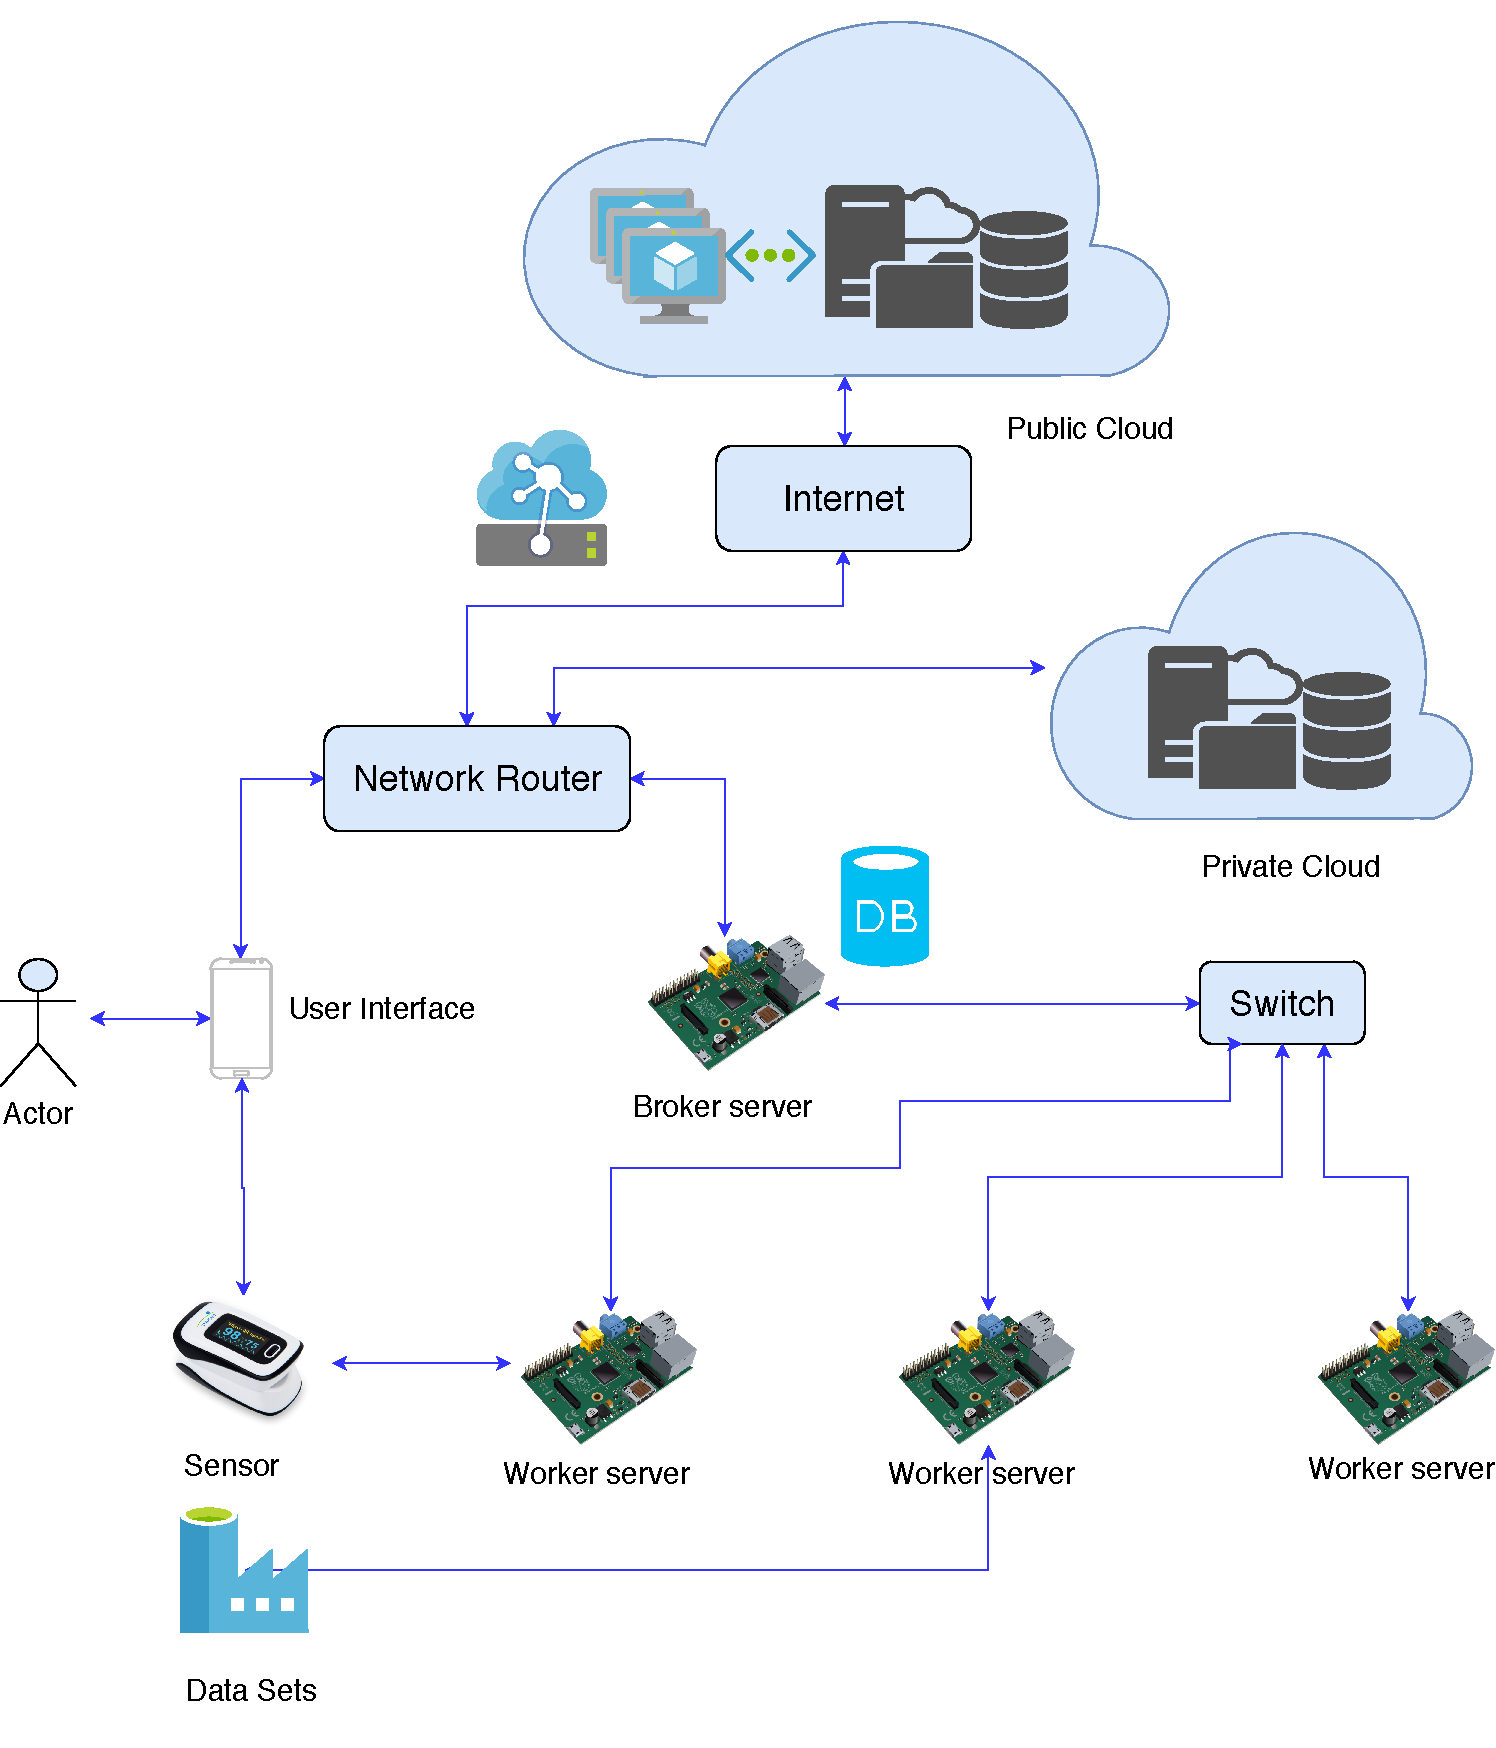
\includegraphics[width=10cm]{network-arch}
\captionof{figure}{Network level structure of the FogBus framework}
\end{figure*}

Figure 1 depicts how different physical components, as described in section 3.2, are connected in the FogBus model. This figure only shows a connection of Broker and worker nodes for one geographical location. The FogBus framework allows \textit{n} number of Brokers for \textit{n} different geographical locations. This \textit{n} can be scaled to large values as described in the next subsection. The User connects his/her device to the local network and interacts with the Master Node using an interface which can be an Android or other smart device. This interface allows communication between sensor/actuator with the Master Node. \\
The Master Node, also referred to as the Broker Node, collects data from the sensor and uses the data itself for analysis or sends it to one of the following:
\begin{itemize}
\item Worker Node in local Network
\item Private Cloud
\item Public Cloud or data center
\end{itemize}
All communication among the Master Node, Worker Nodes, Private Cloud and User is facilitated by the Network Router. Additional workers can be installed in the network using Switches. Communication of the Master Node and the Public Cloud is facilitated with Internet, and the Network Router directs Internet data packets through the connection provided by the Internet Service Provider.\\
The Master Node collects results/actions from the devices mentioned above and send it to user interface or actuator. The master or worker nodes can also receive data directly from data sets and perform actions accordingly. \\
It is in the hands of the user, which service to run and which master to connect to. There can be Master nodes dedicated for specific tasks and in IoT environment multiple services can even run simultaneously requiring connections with multiple masters and/or multiple service running on same master node. 

\subsection{Scalability of architecture}

Scalability of an IoT framework is highly crucial to allow addition of worker nodes easily when the computational demand increases. The traditional Master/Slave system lacks this feature as inherent to it there is one master and several workers connected to the same Master. This can lead to deadlocks when there are several simultaneous requests and the data is being sent to or received by several worker nodes concurrently. To tackle this problem the FogBus framework is based on a model that allows dynamic interconversion between broker and worker nodes to allow scalability on demand. \\
As shown in Figure 2, the FogBus framework allows networks to be scaled by allocating Broker privileges to worker nodes. If many worker nodes are connected to the Broker then some Worker nodes automatically get broker privileges. As shown, initially there are 3 worker nodes connected to the broker. Then, 5 more worker nodes are added. Some worker nodes convert themselves to Brokers and the number of workers per broker reduces from 8 to 2. This approach is possible only because of the platform independence property of the FogBus architecture. \\
This solution for scalability does not hinder with Blockchain management as the blockchains of the Worker Nodes are continued and blockchain verification takes place in the regional network encompassing one Broker and it's Worker nodes. Now, due to multiple Broker nodes that the User can connect to, the tasks can be sent based on the cumulative regional workloads or using a round robin scheme. If by this approach there are several Broker nodes for the User, there can be even more levels that have nodes that act as intermediaries between the user and the broker nodes.

\begin{figure*}[h]
\centering
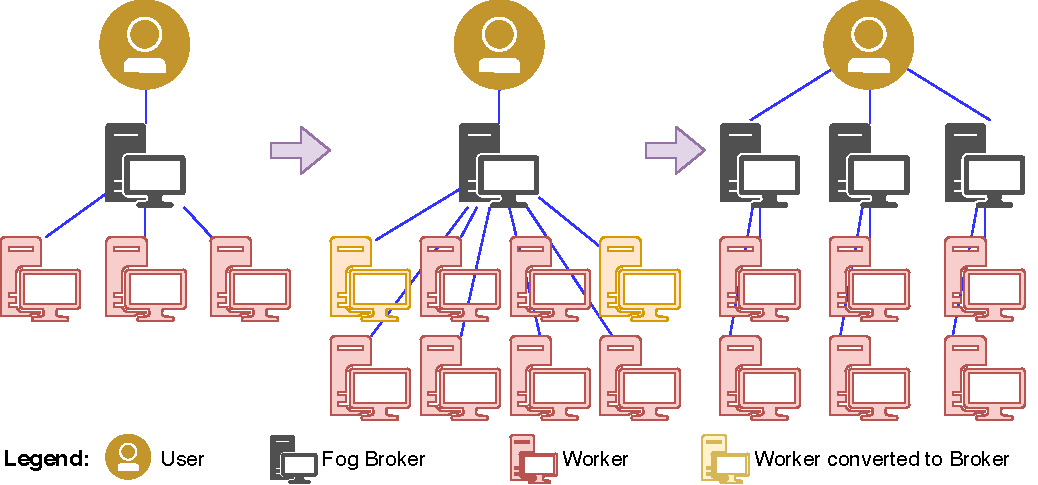
\includegraphics[width=15cm]{scalability}
\captionof{figure}{Scalability in FogBus architecture}
\end{figure*}

\subsection{Sequence of Communication}
A defined sequence of tasks and communication of data helps reduce failure rate and makes it easier to understand the flow of data through the system. Figure 2 below shows the sequence of tasks and data flow in the network.
\begin{figure*}[h]
\centering
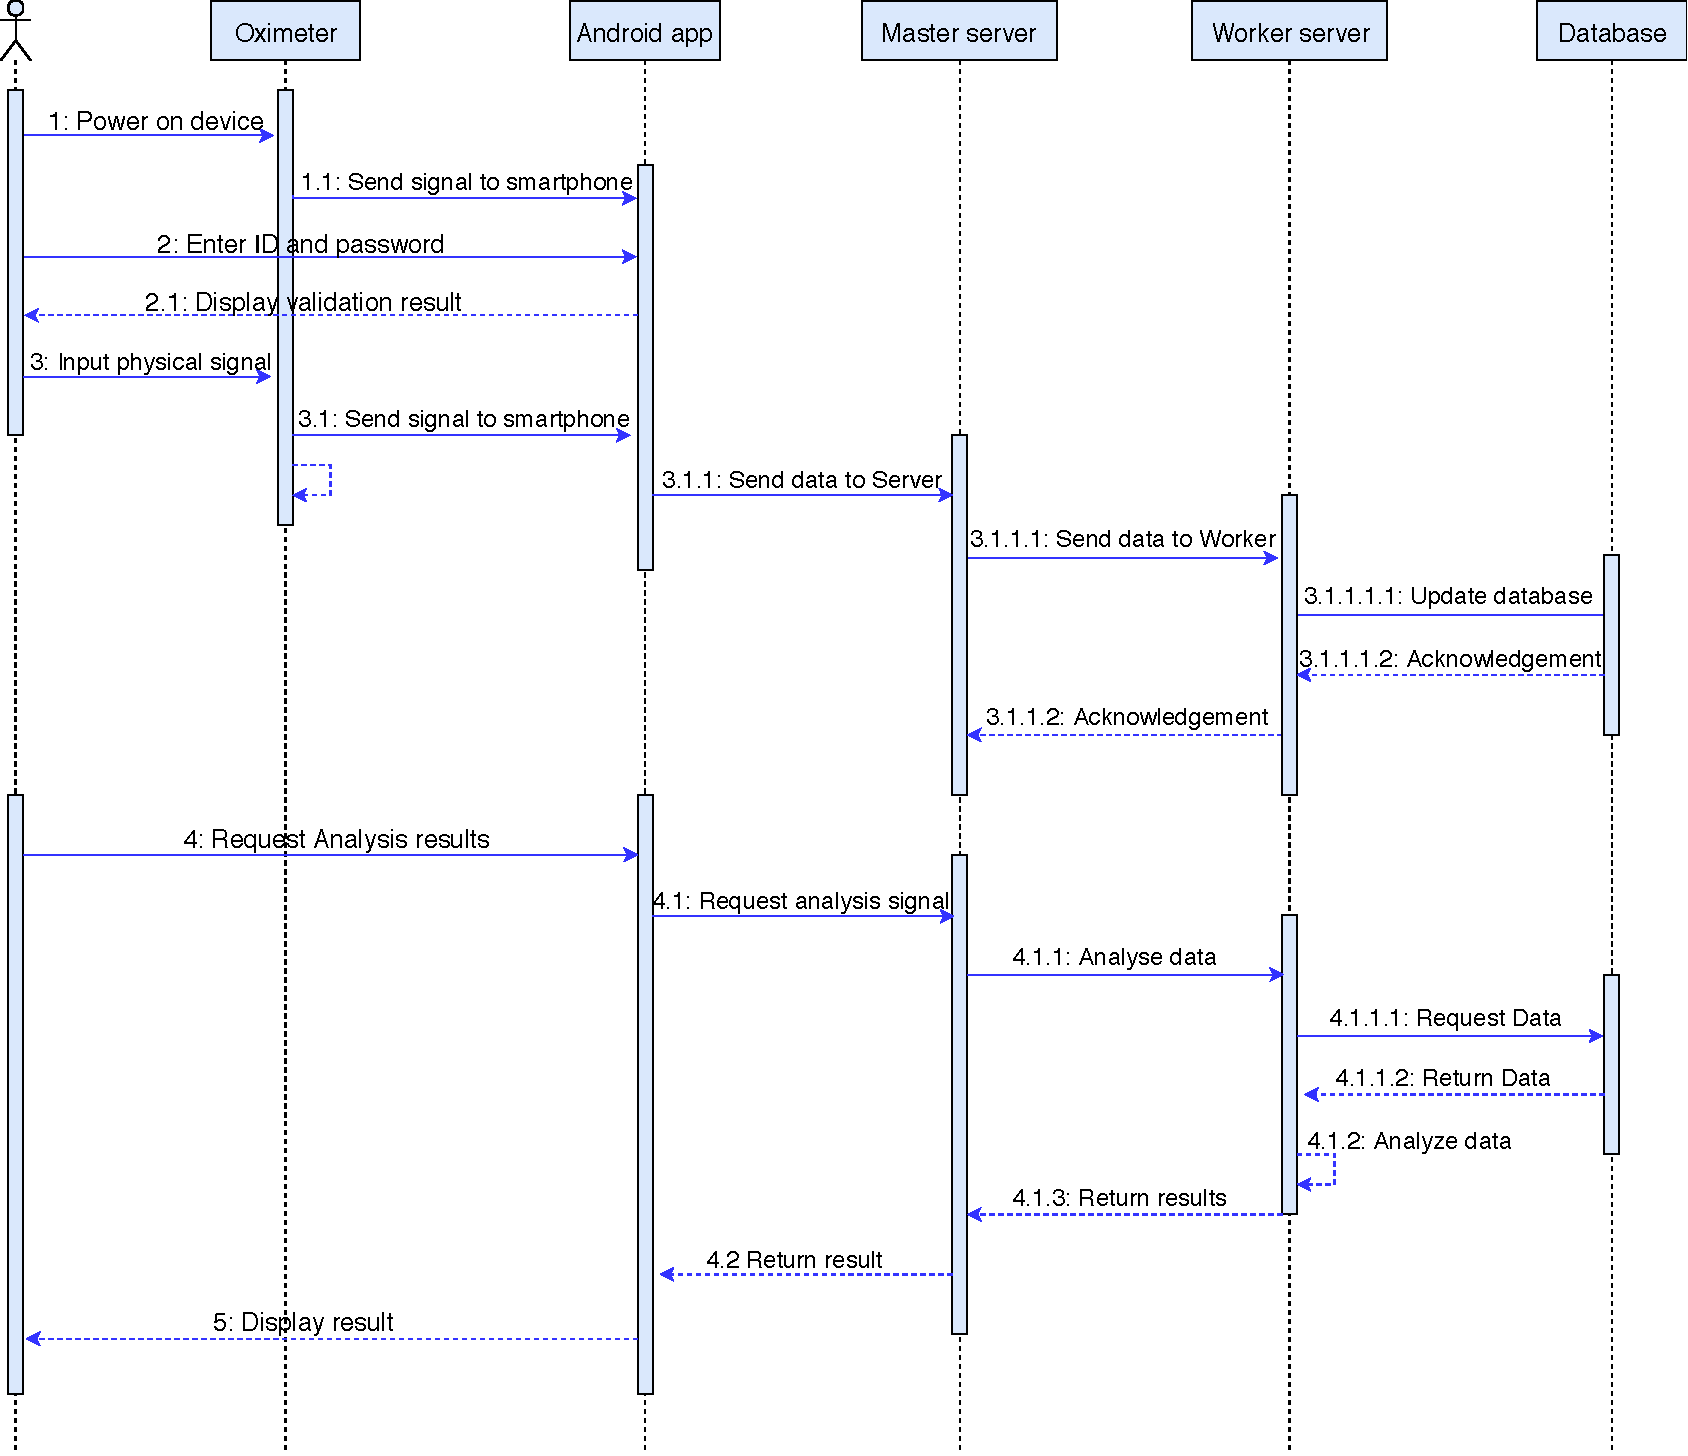
\includegraphics[width=12cm]{sequence}
\captionof{figure}{Sequence of communication among different components}
\end{figure*}

\section{Functional Components}

\subsection{Resource Manager}
As devices at different levels of the network, as shown in the ‘Network Level Model’, offer range of computational capabilities and latencies, it is important to distribute work accordingly to ensure optimum QoS. The devices at the ‘edge’ of the network provide very low latency due to close proximity with the user, sensors and actuators but have tendency to have significantly low computation power and thus higher execution times. The devices far away from users like those on the cloud provide significantly higher latency but due to their much higher computation capabilities provide much lesser execution time. There is thus a trade-off between network propagation latency and computation latency. Depending on different scenarios, different resource management techniques are used.\\
There is scope of considerable reduction of latency caused due to propagation of data if low-computation workload is allocated to edge devices. Even though their execution time would be higher but the critical factor here would be the time caused by data transfer over the network. On the other hand, significant reduction in time can be achieved if high-computation workload is sent to more powerful machines like cloud because in such tasks edge devices might lead to deadlocks and cause the whole system to collapse. \\
The Resource manager of the model should decide the following:
\begin{enumerate}
\item Allocate task to a local worker node or not: As the latency offered by local machines is much lower in terms of the network propagation of data this is a crucial decision to be taken by the master node. Sending to cloud would require considerable overhead and might not be suitable for real-time and mission critical tasks like health-care, robotics, etc. 
\item Allocate task to itself or not: Some small tasks can be performed by the master itself. As the master deals with the load balancing and other tasks like maintaining integrity of data, it might be that the master node is itself busy. Even then some small tasks may arise on rare occasions which require immediate results. At such stages, the master may decide to perform it itself to eliminate data propagation over the network and other authentication and handshaking protocols.
\end{enumerate}
It is a design decision in the implementation strategy how these decisions are taken. Some parameters that are important for taking such decisions include:
\begin{enumerate}
\item \textit{Quality of results}: Each application has its own quality thresholds. As the required quality of results increases, more complex algorithms may be required. Sometimes the algorithm remains same but more number of iterations are required to reach the required confidence threshold. This has a direct impact on the computation difficulty and how well and fast a machine is able to perform repetitive tasks.
\item \textit{Deadline}: The time in which the results are required plays a crucial role in determining the load balancing scheme. As hinted earlier, devices at different levels have different execution times and data propagation times. Based on data flow rate and application runtime it is important to balance tasks among different levels of devices.
\item \textit{Frequency of data sharing}: Closely related to point 2, some tasks might require small amount of data to be analyzed but with high frequency for example -----. In such cases execution time needs to be very low and network bandwidth very high. The device themselves should allow high I/O data flow.
\item \textit{Computation Complexity of Application}: The order of complexity of application determines the number of task request to be sent to cloud. For very high complexity tasks it might me suitable to only use cloud resources to prevent bottlenecking of the software because of low computational capabilities of edge nodes.
\item \textit{Cost of Computation}: Different levels have different currency for computation. Devices over the cloud are metered and are charged based on time of usage. Embedded devices in IoT applications are charged based on the initial physical component cost and then the cost of energy expenditure for functioning of these devices. By normalizing these different currencies using conversion factors, one can determine the cumulative cost for running the framework per unit time/task/user. Inherent to the model requirements, but depending on the scenario, this cost needs to be minimized. 
\end{enumerate}
Different load balancing algorithms can be implemented that specialize in improving some of these parameters based on user needs. A weighted sum of quantifiable factor of each of these parameters and the weights themselves would determine which balancing technique should be used for a specific situation. The \textit{Session Manager} in the Master Node with the help of Workers' \textit{Resource Monitors} handle the resource management in the FogBus framework. See \textit{Implementation} for more details.

\subsection{Blockchain and Digital Signature}
Maintaining integrity of data and ensuring that data is not sent by an unregistered source is very important for the credibility of the system. This is extremely important in systems that maintain real time medical records, financial transactions and other secured platforms. \\
For the integrity of data and prevention from tampering of existing data the model uses Blockchain Technology. Technically, blockchain is a suite of distributed ledger technologies that can be programmed to record and track anything of value. \\
Whenever new data is received by the Master node, it packs it to form a “block”. This block's hash is a SHA256 hash value which is created using the data, block index and a nonce value. The Master node, whenever creating a block mines the block to create a “proof-of-work” which allows the hash to have a particular form/pattern. The Master also creates a random public/private key pair that allow to form a unique signature with the original data. The private key is not shared with the worker node and only data, signature and public key are shared. With this the Worker node is able to verify that the data is from a legitimate source as it saves the public key of the Master node. If any other key is used, that data is rejected. Also, the public/private key pair is kept dynamic per block generation to prevent hackers to generate private key using brute force techniques. Even if one is able to generate a private key for a transaction, it would change for the next and thus become hack proof. \\
The user is also given ability to track the data/block flow through the worker nodes by displaying the latest hashes of the blockchain copy at each node. This ensures that the user is able to see and automatically take action on which nodes are more prone to attack and/or are being targeted by hackers.\\
Thus:
\begin{enumerate}
\item Dynamic Public and Private Key Generation
\item Digital Signature Verification
\item Blockchain maintenance and validation
\item Proof of work sharing and verification
\item Automatic majority chain deployed in minority workers
\item User displayed the latest hashes of each node
\end{enumerate}
Points 1 and 2 ensure that the data recorded is from genuine source and points 3, 4 and 5 ensure data integrity. The \textit{Master Interface} and \textit{Worker Interface} modules in respective nodes handle the blockchain and signature verification in the FogBus framework. See \textit{Implementation} for more details.
\begin{figure}[h]
\centering
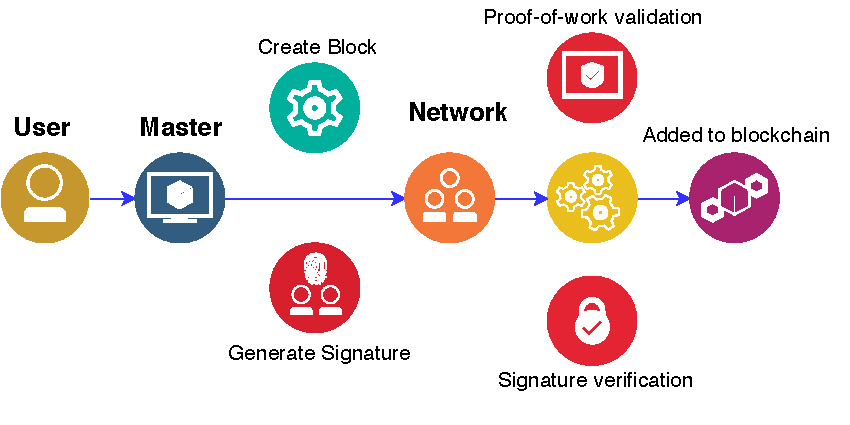
\includegraphics[width=9cm]{blockchain}
\captionof{figure}{Blockchain concept level diagram}
\end{figure}

\subsection{Data Input/Output}
There exist several ways of interacting and sharing data from sensors and among fog nodes. It is crucial that this data sharing mechanism is failsafe in terms of data theft and fraudulent manipulation. The streams of data can also be dedicated. Another important part is that the protocol followed for communication among fog devices should be supported by all nodes, complex and rarely used encryption standards may restrict diversity of devices that can be used. \\
The sharing of data with sensors and actuators needs to be as close to real time as possible. For mission critical application proper data transfer frequencies are important. For the case of static transfer frequencies, very high frequencies can lead to computation lag from the worker nodes, very low frequency can cause reduction in the Quality-of-service (QoS). \\
The current model uses HTTP protocol for communication between different nodes in the local network and the Aneka’s protocols for task distribution to cloud and other devices. All data is currently transferred in plain text using the HTTP REST APIs specifically GET and POST. The \textit{User Interface} and the \textit{Session Manager} collectively handle the Data I/O in the FogBus framework. See \textit{Implementation} for more details.

\subsection{Computation over Data}
Another important criteria for model development is that it is generic in terms of the service it provides. In the IoT world there are several applications in which Fog, Edge and Cloud Computing can be used, and there are several others that haven’t even been thought of. It is important that the frame work allows services to be used that can be changed, modified and/or extended easily. \\
The computation/analysis requirement of the service also affects the Resource management policy and data transfer rate requirements. Based on different services and end-user requirements, performance metrics can be designed and the framework can be optimized accordingly.\\
The model uses Java runtime environment for data analysis due to its ability to be run in diverse machines. The \textit{Analysis Application} in the Workers does the computation over data. See \textit{Implementation} for more details.

\subsection{Data Storage}
Many applications require data to be stored for future use. This data being shared among multiple nodes is prone to attacks. It is thus important to implement strategies/techniques that keep data resilient and prevent it from tampering. Not only keeping saved data secure is important, but the methods used for data extraction and sharing among nodes is also a concern. The \textit{Network} and \textit{Session Managers} handle the data storage in the FogBus framework. See \textit{Implementation} for more details.

\section{Implementation}
The software has been built using platforms that are supported by a wide range of devices including those used for IoT application. The main software is divided into four different components:
\begin{enumerate}
\item Interface Web Scripts (Based on PHP)
\item Blockchain Interface (Based on Java)
\item Aneka analysis code (Based on C\# and .NET)
\item Analysis Jar file (Based on Java)
\item User Interface (Android Application, or web-based interface)
\end{enumerate}
The web scripts require an Apache server to be set up in all nodes and MySQL server in master. Each of these have different roles and are distributed among different nodes. All local network and public cloud interaction is based on Blockchain to prevent hackers from accessing and manipulating data.\\
Interaction with the user plays a key role in obtaining the user requirements and also acts as an intermediary between the network and sensors/actuators. It is crucial for the user interface to be accessible from a wide range of devices and be friendly for interaction. Some requirements of this interface include:
\begin{itemize}
\item Set the architecture of the network in terms of worker nodes
\item Connect to Sensors and actuators for real time data sharing
\item Allow modification and extension of different components for application specific optimization
\item Ability to set/modify the resource management policy
\item Display/Modify/Erase data collected
\item Enable or Disable Master as a worker
\item Enable or Disable Aneka tasks to be spun
\end{itemize}
The current implementation of the FogBus model uses PHP based web scripts as an interface with the user and also backend interface among master and worker nodes. An abstract level depiction of the implementation is shown in Figure 4.
\begin{figure*}[h]
\centering
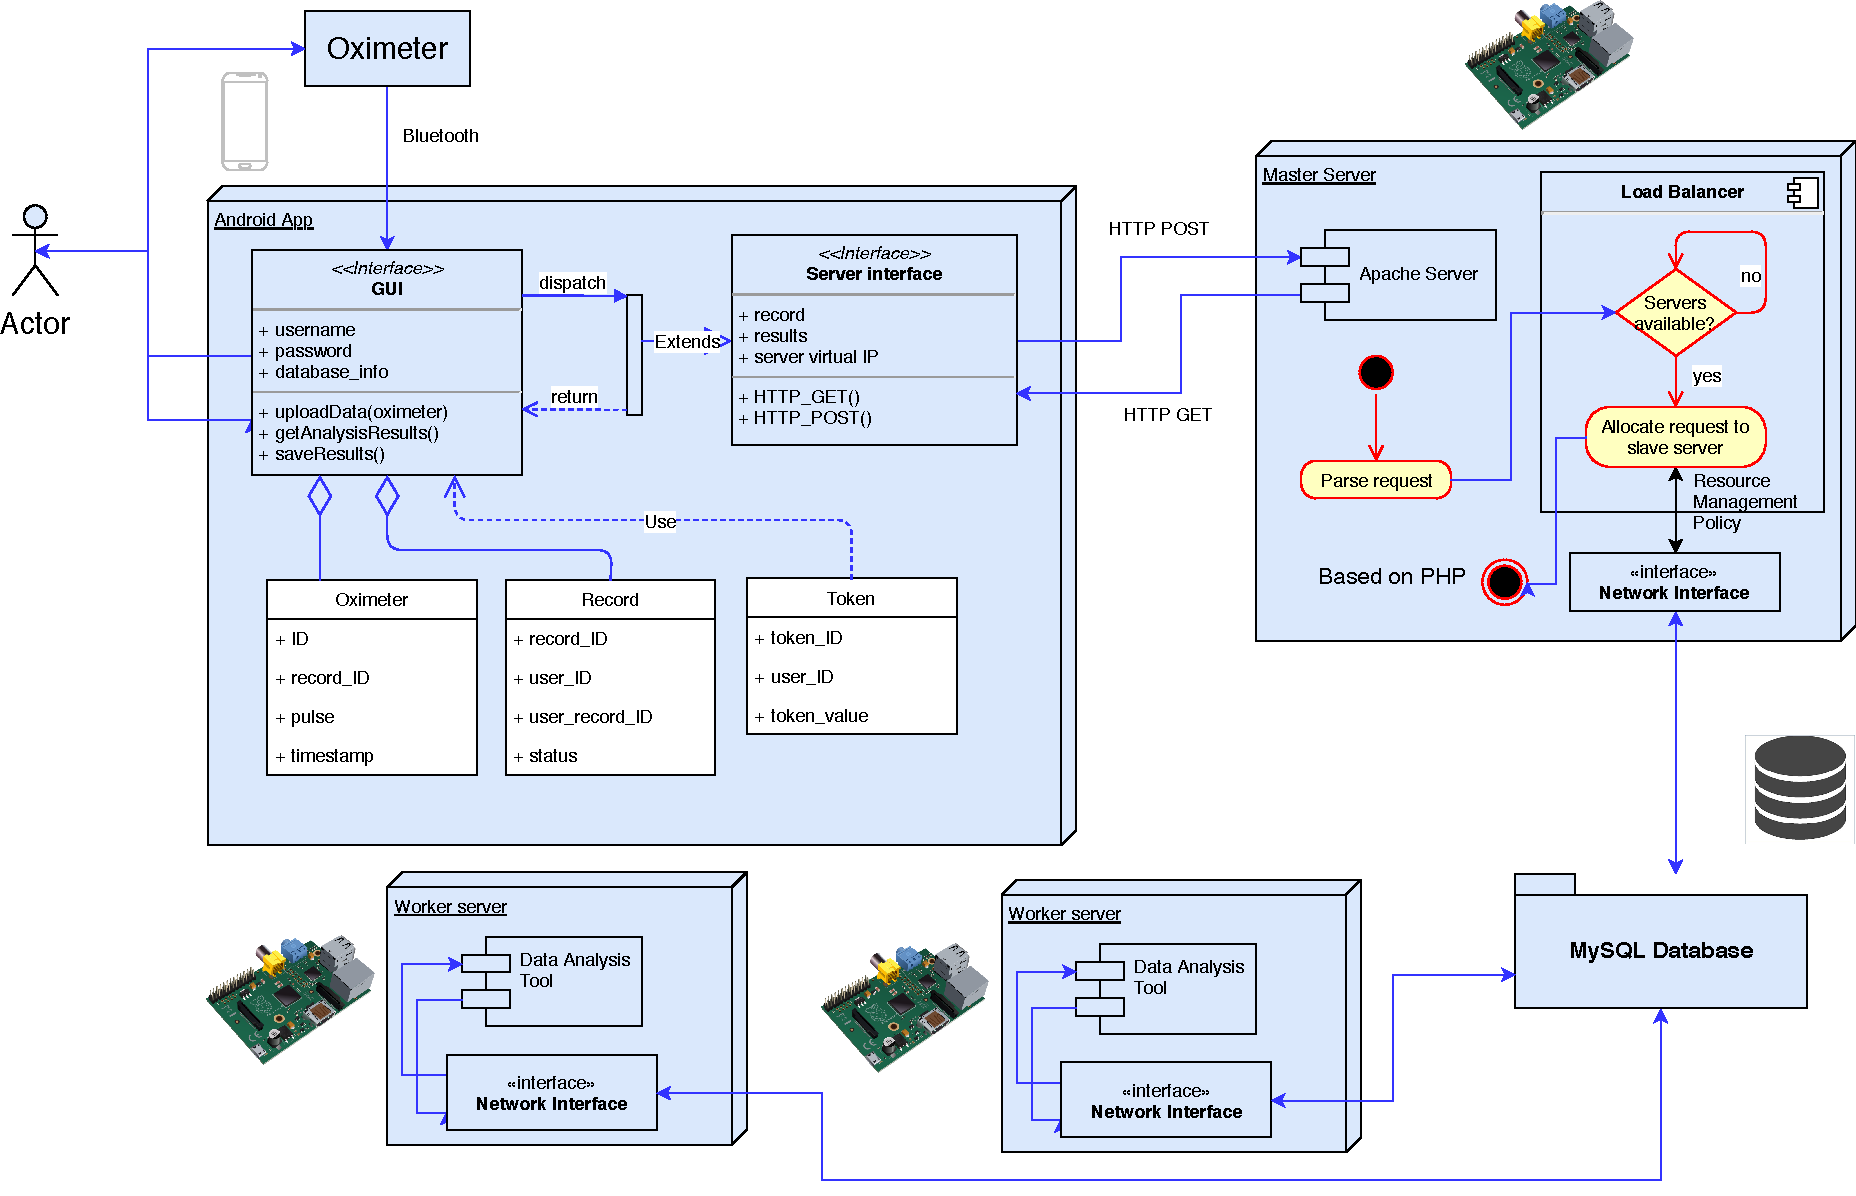
\includegraphics[width=\textwidth]{model-with-interface}
\captionof{figure}{Sequence of communication among different components}
\end{figure*}

Java and PHP (based on HTTP) have been chosen for all local interface because they are cross platform languages. Compiled Java program runs on all platforms for which there exists a JVM (Java Virtual Machine), which includes large number of Operating systems (Windows, Linux, Mac OS X). PHP scripts can run almost everywhere (Unix, Windows, Linux, Embedded Systems, Risc, NetWare). Most embedded and IoT devices come with networking protocol stacks for HTTP communication, and can be easily installed in those that don't. \\
Due to the cross platform nature of the languages used to develop the FogBus framework, it can be deployed in a plethora of devices.

\subsection{Master Node}

The framework at the Master Node side can be described in terms of following major modules.

\subsubsection{Login Verification Module}
This module takes the user login credentials and verifies them with the database. An HTML form allows users to input login information including username and password is displayed first. This form takes in the login information and sends it to Master node using the POST method. The script then checks the input information with the MySQL Database. Using the \textit{mysqli\_connect} command, the database name and table name are verified. After the form, the database and table connection success are shown on the web page. 
The login information is checked using the SQL query to find entry with the given details. If the number of returned rows is greater than 0 then the login is successful and page navigates to Navigation Module. If the login details are not found in the table then a prompt is displayed to allow re-entering the login details. 

\subsubsection{Navigation Module}
This acts as a menu or navigation page for the user and allows user to go to either the Network Manager or the Session Manager.

\subsubsection{Network Manager}
This module manages all the worker IPs for the Session Manager. It maintains the configuration file in which every line contains one IP address of a worker. The configuration file also holds whether Master and Aneka could be given the task of analysis or not. A reset command allow the configuration file to be reset to default state where there are no registered worker IP addresses and both Master and Aneka are enabled for task processing. 
Whenever a new IP address is set it is appended to the configuration file. \\
Another task performed by the Network Manager is to synchronize the Jar file used for analysis. This service sends a request to the manager page of each worker node to synchronize the executable jar file from master. The worker node then downloads the master’s copy of the executable and overwrites its own with it. 
This Manager also lets user configure other worker nodes automatically by sending it’s IP address and latest public key to other nodes for updating. The configuration files of the worker nodes is updated and manual configuration update is not required.

\subsubsection{Session manager}
This module performs the most of the software functionalities.. The user can manually input the data for send data via the GET request to the master node. After inputting the data, if the “Analyze” button is clicked, then the content of configuration file is parsed to obtain list of worker IP addresses. \\
Variables \$toMaster and \$toAneka store if the task is to be given to the Master or Aneka or not. This module also handles the “Fail over” and “Load Balancing” schemes of the software. The variable \$ips is an array of the IP addresses and \$loads is their corresponding loads. The PHP method file\_get\_contents() allows us to get a string form of the webpage passed as the argument. An error operator lets it return FALSE in case of errors. If any HTTP request for load returns FALSE then variable \$my\_var is set to 100, and error message is displayed on the screen. Setting load to 100 has the effect that this node would never get the task and hence removed from load balancing IPs. The next time the worker IPs are accessed for load, this is checked again and if the particular worker node is available, it is taken into the load balancer. \\
Using a for loop, the \$loads array is populated by accessing the Resource Monitor of the workers corresponding to the IP address. If the load of any worker is < 80\%, then the variables \$toMaster and \$toAneka are set to false. In effect, when master is enabled as worker, this sets \$toMaster to true only when all worker nodes have more that 80\% load. Same is the case for Aneka container. If the task is not given to the master or Aneka, i.e. \$toMaster and \$toAneka are false, then the IP of the worker with minimum load gets the task. The task is sent using the GET method to the Worker Module of the worker with that IP address. Otherwise, randomly either the master or Aneka gets the task. If the task is sent to master, then it is sent using GET method the Worker Module in the local machine. If the task is sent to Aneka, then it is sent using the GET method to the Aneka Interface. \\
The load balancing strategy used is shown in Figure 5.
This module also sends the block details to the other worker nodes. It saves the data received from the sensors to a data file which the Master Interface java application uses to form a new block. The new block hash values and proof-of-work with public key and signature are shared to each node for updating blockchains. If any node reports error in terms of blockchain tampering or signature verification, then the blockchain in majority of the network is copied to that node.
\begin{figure}[h]
\centering
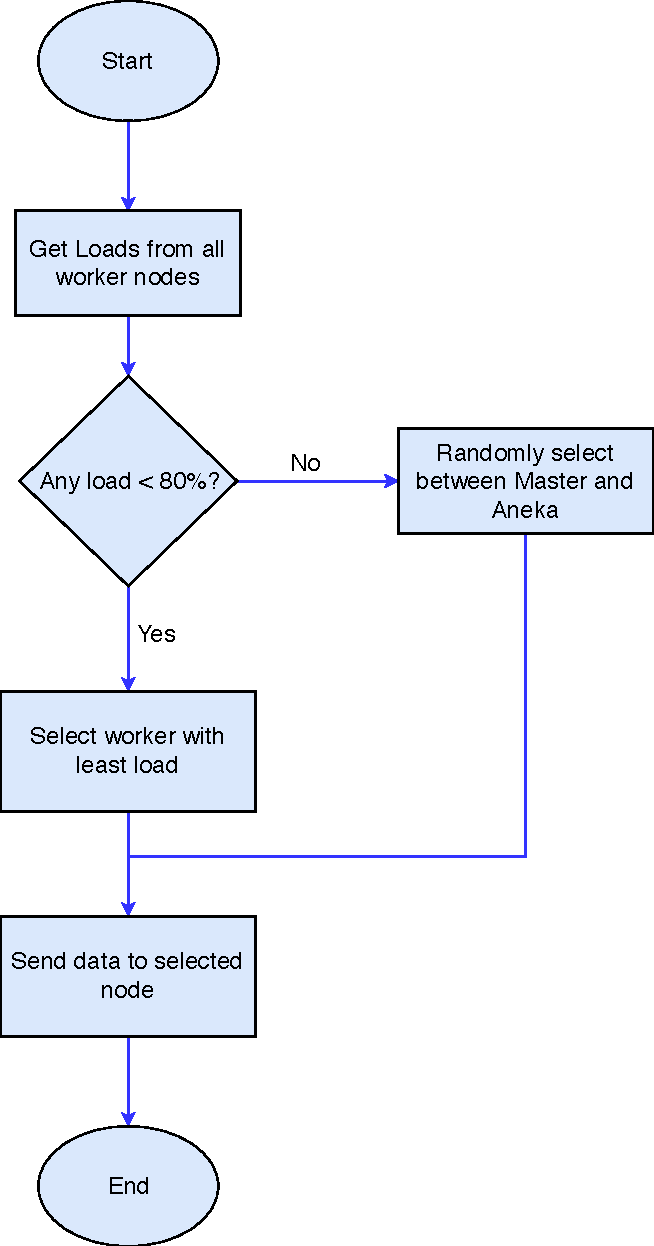
\includegraphics[width=5cm]{load-balancing}
\captionof{figure}{Simple Load balancing scheme implemented in code}
\end{figure}

\subsubsection{Master Interface}
This module acts as the blockchain interface for the Master node. It forms new blocks and generates random public/private key value pairs and shares with worker nodes. It also maintains its own blockchain and sends data, hash values and proof-of-work to other nodes for verification. All hashes are generated using SHA256 algorithm and data transferred in Base64 encoding.\\ 
Each block also maintains it’s timestamp of creation for backtracking and validation of chronological sequence of block creation in the chain. This helps in checking if a block created later in time has not been inserted in between in fraudulent manipulation. \\
The received results from the worker node are displayed on the webpage and a cumulative graph shows all the data that has been recorded since the user was registered. 

\subsection{Aneka}
The framework at the Aneka side can be described in terms of following major modules.

\subsubsection{Aneka Interface}
This Module acts as an interface between the Aneka software and the master session script. It receives data to be analyzed from the session script and saves it to the data file. When analysis is complete, the contents of the result file are displayed on the webpage to be parsed by Master Node.\\ 
When the Aneka software gets the data for analysis it itself decides to which container the data needs to be sent if it is a Task based implementation or can be sent to multiple containers when in Thread based implementation. 

\subsubsection{Aneka software}
The Aneka code (in C\#) parses the data file every 500ms and checks if pending analysis exists. If yes then it forms Aneka tasks/threads and launches it to other Aneka containers which might be on the cloud or in local network. \\
Here also blockchain has been implemented to ensure data integrity and secure the data and results from hackers. Whenever a new thread or task is spun, the proof of work is calculated by the master node and is sent to other nodes for verification. If verification passes then the block of data is added to the chain, otherwise the data is discarded. Each time new task is sent, the chain is validated by checking the correctness of the last block’s hash value and matching the previous hash value of the last block with the hash value of second last block. \\
Digital Signature management has also been implemented so that data from unknown sources can not be added to the blockchain, thus ensuring no outside and unwanted manipulation can be done. Each Aneka node is given a public and private key. The signatures are formed using private key and verified using public keys. 

\subsection{Worker Node}
The framework at the Worker Node side can be described in terms of following major modules.

\subsubsection{Resource Monitor}
It is a PHP based module that keeps a real time information of the load on the worker node. This Monitor is accessed by the Master Node for it's load balancing scheme implementation. 

\subsubsection{Network Manager}
The worker’s manager page allows user to set the Master IP address which is used for synchronizing the executable Jar file. It also displays the current set IP address of the Master which is saved in the configuration file and the analysis file name that is being used for computation on the data. The Network Manager also keeps track of the Master Node's public key that is used to sign the data sent to the worker.

\subsubsection{Worker Module}
This module receives data to be analyzed using the GET method. It acts as an interface between the Master Node and the Java based analysis application.

\subsubsection{Analysis Application}
It performs the computation on the data sent by the Master node and sends results to the Worker Module to be forwarded to the Master Node. 

\subsubsection{Worker Interface}
This Module takes in the updated block details from the master node, analyzes them and adds them to it's blockchain if validation checks pass. If the Worker Interface application throws any exception in terms of data tampering or signature verification, it is reported to Master node. Data validation includes the following checks:
\begin{itemize}
\item Checking the source:
\begin{itemize}
\item Public Key received matches the registered public key of master node
\item Signature Verification of data received with the public key
\item The tuple of data, public key and signature is not same as last
\end{itemize}
\item Checking the block:\
\begin{itemize}
\item Hash of the block matches the calculated hash value
\item Proof-of-work follows the required pattern
\item Previous hash corresponds to the hash of the latest block
\end{itemize}
\end{itemize}
If the source verification fails then block is ignored and data breach is informed to the master node. If block details check fails then the errors are reported to master. If the block is valid, it is added to the blockchain and no errors are reported to Master.\\
Thus, a hacker can not add new data or tamper with existing data due to the following argument:
the hacker can manipulate with data only in the following ways:
\begin{enumerate}
\item Add new data (and different from last)
For adding different data from the last one the hacker would need to develop a tuple of data, public key and signature that pass the signature verification test and match with master public key. Two sub cases arise:
\begin{itemize}
\item He/She can not use the same public key as the last sent data to develop a signature, he/she would require the private key of the master which is hidden. To reverse engineer the private key of the master using brute-force requires an unfeasible amount of computation power. Thus, the signature verification step ensures that this case cancels out.
\item He/She can not use some random private key as then the public key won’t match with that of master. The step that matches the public key with that of the master node ensures that this case also cancels out. 
\end{itemize}
\item Add new data (same as last)
\begin{itemize}
\item For adding new data which is same as last the hacker can easily keep using the same tuple of public key, data and signature. This is very much probable for causing deadlocks and DDoS attacks, but due to the check performed by \textit{Worker Interface} which rejects repeated blocks, this is not possible (the \textit{Master Interface }ensures that every new block has at least one of public key, signature or data different from previous block)
\item Hacker cannot use different public key and signature for the same data as then the Master public key check would reject it.
\end{itemize}
3.	Tamper existing data \\
When the validation of blockchain is performed the following checks at the \textit{Worker Interface} report data tampering:
\begin{itemize}
\item Hash of the block matches the calculated hash value
\item Proof-of-work follows the required pattern
\item Previous hash corresponds to the hash of the latest block 
\end{itemize}
\end{enumerate}
If data is tampered with, the one of these checks would report the manipulation as the hash of some block would not match pattern if not mined. Even if that particular block is mined, then the previous hash value of the next block won’t match the hash of this block, so each and every block of the chain after this block needs to be mined. This is a very computation intensive task. Moreover, if the hacker is able to mine all blocks in the chain, in the next transaction the last hash value of this chain would be different from others and the chain would be rejected. So, the hacker would have to take control and mine simultaneously more than 50\% of the network blockchains which is not possible.

\begin{figure*}[h]
\centering
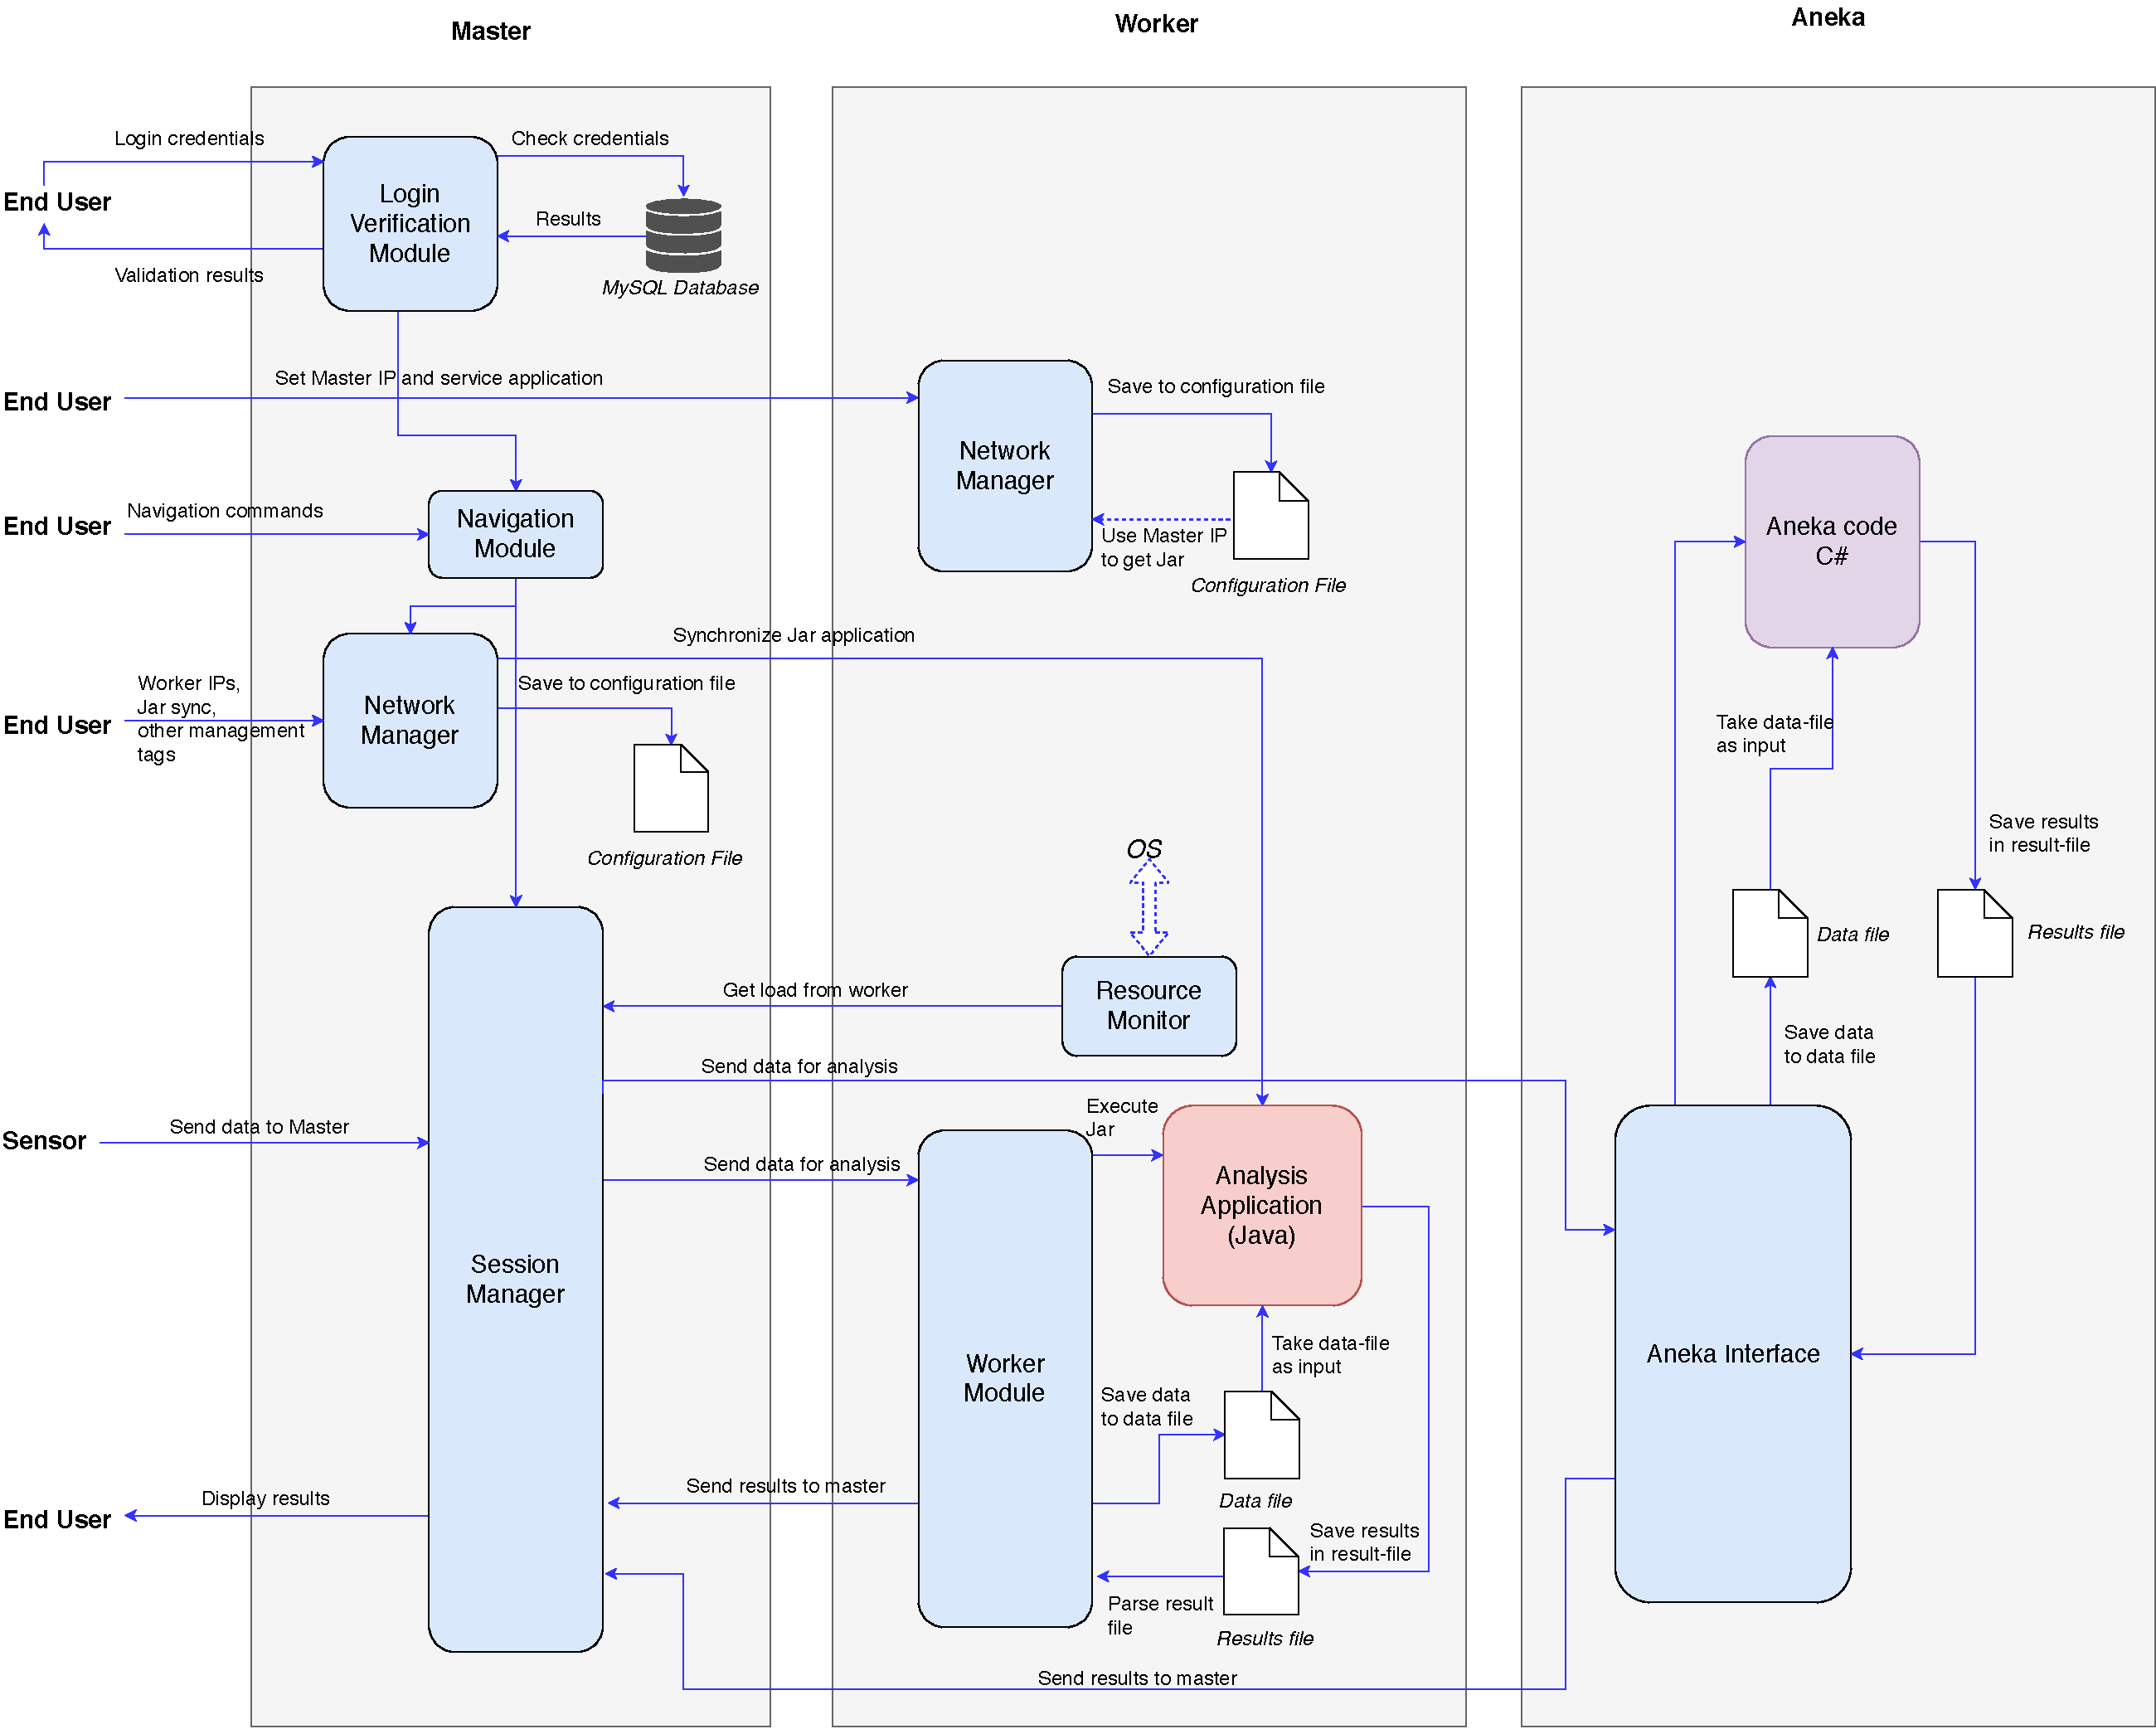
\includegraphics[width=18cm]{working}
\captionof{figure}{Complete working explanation of the analysis tool}
\end{figure*}

\section{Application Case Study : Sleep Apnea Analysis}
The FogBus framework has been deployed and tested with a real-life application: Sleep Apnea Analysis. Sleep Apnea is a disease in which air stops flowing into the lungs for 10 seconds or longer while in sleep. This reduces the oxygen level and sensing that the patient has stopped breathing, the brain triggers to wake up just enough to breathe. In some cases, this can happen over 30 times in an hour. Many people have sleep apnea, (also known as sleep apnoea) but may not even know it. In fact, sleep apnea affects more than three in 10 men and nearly two in 10 women, so it's more common than you might think. \\
Sleep Apnea analysis is very difficult and cumbersome. An overnight or laboratory-based sleep study requires you to stay overnight at hospital in a sleep unit or laboratory usually consisting of a number of private, quiet, single rooms.  You will sleep with sensors hooked up to various parts of your body.  Physicians usually recommend this test for more complicated or difficult to diagnose cases.\\
The doctors use a term Apnea Hypopnea Index (AHI) and the Electrocardiogram (ECG) data to diagnose if a person is suffering from Sleep Apnea or not. Using open source algorithms, we deployed an analysis application that could analyze data from a Bluetooth enabled Pulse Oximeter and give diagnosis results based on the data.\\
This was divided into two parts: Data analysis application and the Android Interface with Bluetooth Oximeters.

\subsection{Physical Infrastructure}
The devices on which the FogBus framework was deployed:
\begin{enumerate}
\item Master Node: Dell XPS 13 laptop, OS: Windows 10 
\item Worker Node: 2x Raspberry Pis, OS: Raspbian Stretch
\item User Interface: Android Device, OS: Android 8.0
\item Sensor: Pulse Oximeter, Data encoding UTF-8
\item Public Cloud: Microsoft Azure B1s Machine, OS: Windows Server 2016
\end{enumerate}
All nodes and android device were connected using a local hotspot.

\subsection{Data Analysis Software}
References: \\
https://github.com/subrahmanyamanigadde/sleepapnea \\
https://github.com/monarch-initiative/sleep-apnea-clustering \\
The sleep apnea analysis app was developed using a combination of the above two open source repositories.  \\
The analysis application takes the data file as input and stores results in the result file. When new data is found in the data file, it parses it and splits the string with “,” as a delimiter, and converts all strings to integers. Two data sets are parsed in this way: heart rate and blood oxygen level. For oxygen level, in a broad sense, the analysis is done in the following way: 
\begin{itemize}
\item There is a dip Boolean variable, which stores whether there is a dip in oxygen level, a count which stores the number of times dip changes to true and a min which stores minimum oxygen level 
\item Whenever the oxygen level goes below 88, dip turns to true and stays true till oxygen level 
\end{itemize}
comes above 88. This is verified with an increase in the heart rate corresponding to or with an offset with the timestamps along a dip in oxygen level.
\begin{itemize}
\item This count becomes the AHI (Apnea - Hypopnea Index), used to determine the disease severity
\item Based on standard thresholds, the disease probability of the sleep apnea is determined 
\end{itemize}
For the heart rate data, the analysis is done using the following method:
\begin{itemize}
\item The Minimum and Maximum heart rates are determined in the input data
\item The average heart rate and average rise or fall of the heart rates is determined
\item Those close to the dips in oxygen level are filtered
\item Based on some thresholds the ECG diagnosis is determined
\end{itemize}
Using both the diagnosis results, disease severity of the patient can be evaluated.

\subsection{Android Interface}
References \\
MIT App Inventor: http://appinventor.mit.edu/explore/front.html \\
App Inventor JavaBridge: http://www.appinventor.org/jBridgeIntro \\
The android app (named “HealthKeeper.apk”) allows the android device to act as an intermediary between the Oximeter sensor and the Master server. Rather than sending data manually through the GET HTML form, this app records and sends data automatically. The app has been developed on an open source platform: “MIT App Inventor” which can be seen at this link. The source file for the android applicatoin can be found \href{https://drive.google.com/open?id=1rPIf_NHuBXp6peUX3vkzqJg5hfht3KDC}{here}. The application is divided into two screens namely: Welcome screen and Session screen. The Welcome screen asks user to pair the Bluetooth Oximeter with the Android device and enter the Master server’s IP address. \\
The \textit{masterip} is the global variable which stores the IP address entered by the user. The list global variable stores a list of \textit{masterip} and Bluetooth device address. The \textit{PairSensor} is a list picker to select from the available bluetooth devices. After picking, the BluetoothClient connects to the selected address and displays it on the screen. When the “Connect” button is clicked, the list objects are appended and sent to the Session screen. Based on the make of different oximeters, the corresponding service and characteristic UUIDs are used. \\
The Session screen is the main screen that handles all interaction with the master server. The blocks below show the variable initializations. The data variable stores the data received from sensor in list form, \textit{loop} variable is a boolean for timer, and \textit{url} variable stores the web address of the master node’s index page.\\
The “Refresh” button connects the “WebViewer” to the url. When the "Start Recording" button is clicked, the timer is reset, the BluetoothClient connects to the address and starts collecting data from the sensor till the "Stop Recording" button is clicked. When the Stop Recording button is clicked, the timer is stopped. When Analyze button is clicked, the data is submitted for analysis and results displayed on the WebViewer. The analysis function is shown in Figure 6, which Connects the WebViewer to the Session Manager with GET request: analyze value set, which ensure that data is submitted for analysis.

\begin{figure}[h]
\centering
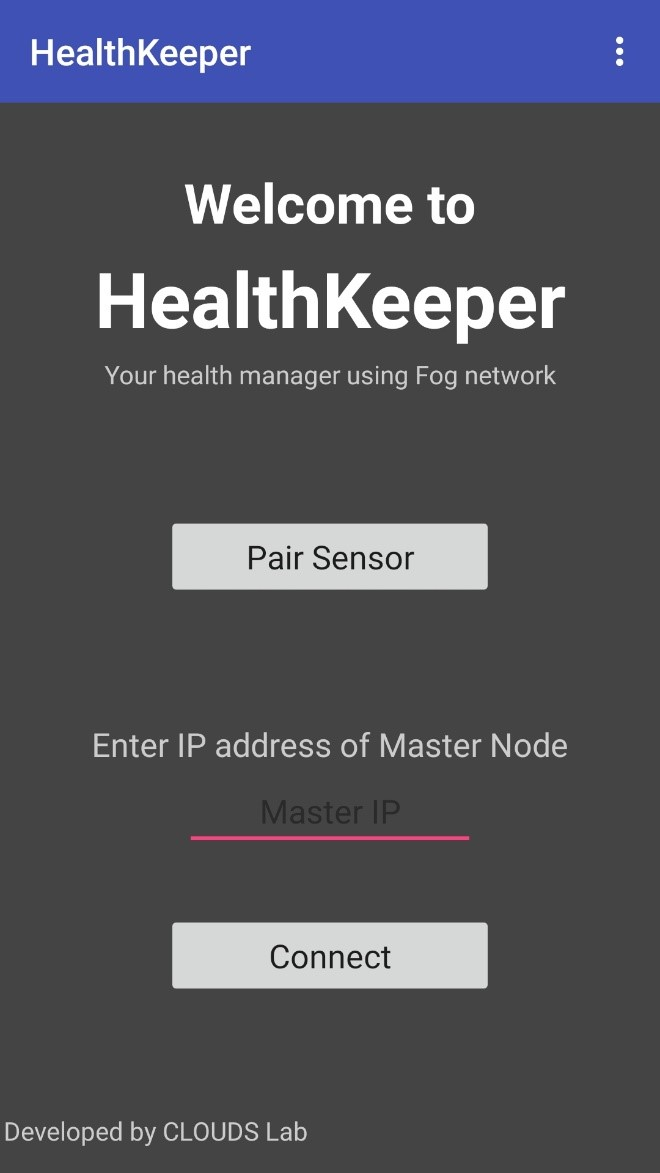
\includegraphics[width=4cm]{welcome}  \ \ \    
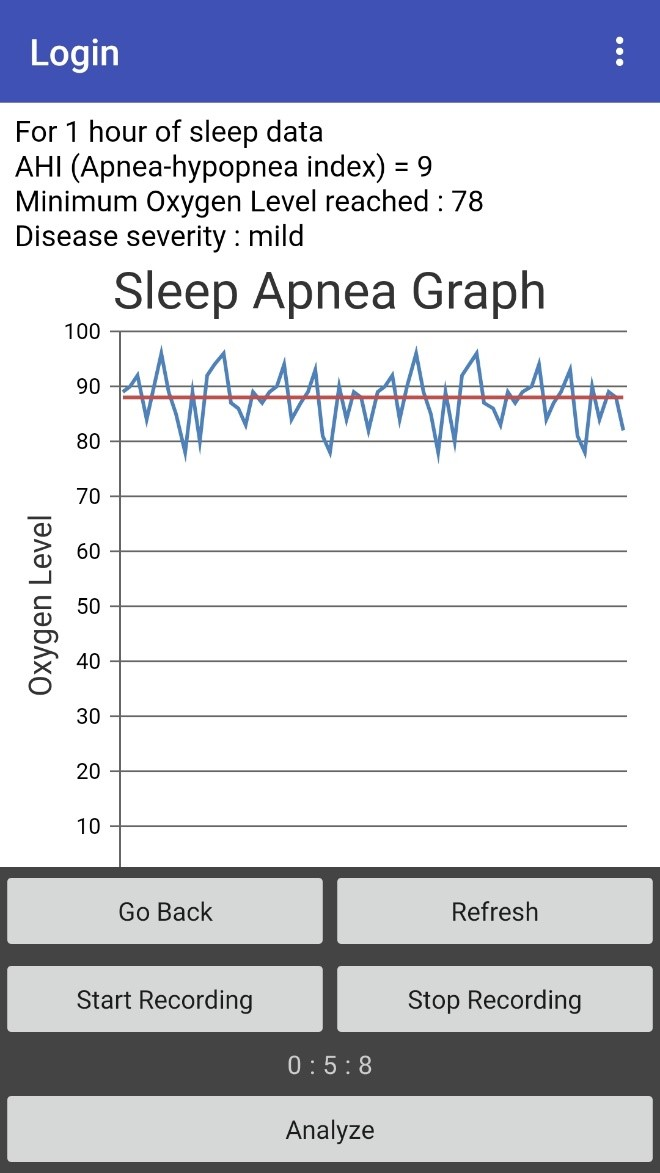
\includegraphics[width=4cm]{session}
\captionof{figure}{Welcome and session screens of the Android Application}
\end{figure}

\section{Performance Evaluation}

In this section we have tested the FogBus framework with the Sleep Apnea Analysis case study on different scenarios. Each scenario was built using a combination of the following test case options:
\begin{enumerate}
\item \textit{Maximum Load / Constant instruction rate}:  In the maximum load case, next task was sent as soon as the previous task was over to ensure that the FogBus framework is continuously on work and has no idle time. The 'Maximum Load' case can also be called as 'No Interval' case. In the constant number of instructions case, every task was sent at a gap of 5 seconds. It can also be called as 'With Interval' case. This would mean a total of 60 tasks (for a 5 minute test) but due to the overhead of master node and network propagation 60 was the maximum limit.
\item  \textit{With / Without Blockchain}: As the names of scenarios suggest the test cases were based on whether the blockchain security was enabled on not. If the blockchain is disabled there is a significant reduction in latency, network usage, and energy consumption.
\item \textit{Fog Only / Cloud Only / Master Node Only}: This was whether the tasks were sent to only the Raspberry Pis or Azure through Aneka or Master itself performed all computation.
\end{enumerate}
As the test configurations were built as a combination of these test case options, the total number of configurations were $2 \  \times \ 2 \ \times \  3 \ =\  12$. Each configuration was tested for 5 minutes as the following parameters were observed and recorded:
\begin{enumerate}
\item Number of tasks performed in 5-minute duration
\item Power consumption (Master + workers + Azure)
\item Energy per task (Master + workers + Azure)
\item Bytes sent / second by master
\item Bytes received / second by master
\item Network usage per task (Based on the bytes sent + received per task)
\item Average task latency (i.e. the time duration between when the master sends data for analysis to worker/Aneka/itself and when it gets results)
\item Master CPU Usage \%
\item Master RAM Usage \%
\item Master Cache Usage
\end{enumerate}

The data parameters were recorded using Microsoft Performance Monitor$^\copyright$ at the Master and Azure machines, and using NMON Performance Monitor at the Raspberry Pi. The green bars in graphs are for Fog Only case and blue bars are for Cloud Only case. Each task had two data sets: Oxygen level and Heart rate, each data set having 15 integer values.

\subsection{Number of Tasks}

The number of tasks performed in a constant duration of 5 minutes can be seen in the graphs for the different cases. We observe that the Number of tasks is higher in the Fog Only case than the Cloud Only case. For the Maximum Load case (i.e. tasks sent with no interval) the number of tasks that are performed depends on the Network propagation and time required by the node to perform analysis. We know that the network propagation time is lesser for fog devices, and execution time is lower for cloud. As the results show us, the latency is lower for the Fog Only case compared to the Cloud only case, and as $Latency\ =\ Network\ propagation\ time\ +\ Execution\ Time$, it is apparent that the difference in network propagation times in fog and cloud cases is more than the difference in computation time. This shows that the Fog Only case is better for performing high number of tasks.\\
We also see that without blockchain the framework is able to perform much higher number of tasks. This is because of lower workload and lesser amount of data to be shared among nodes.
\begin{figure}[h]
\centering
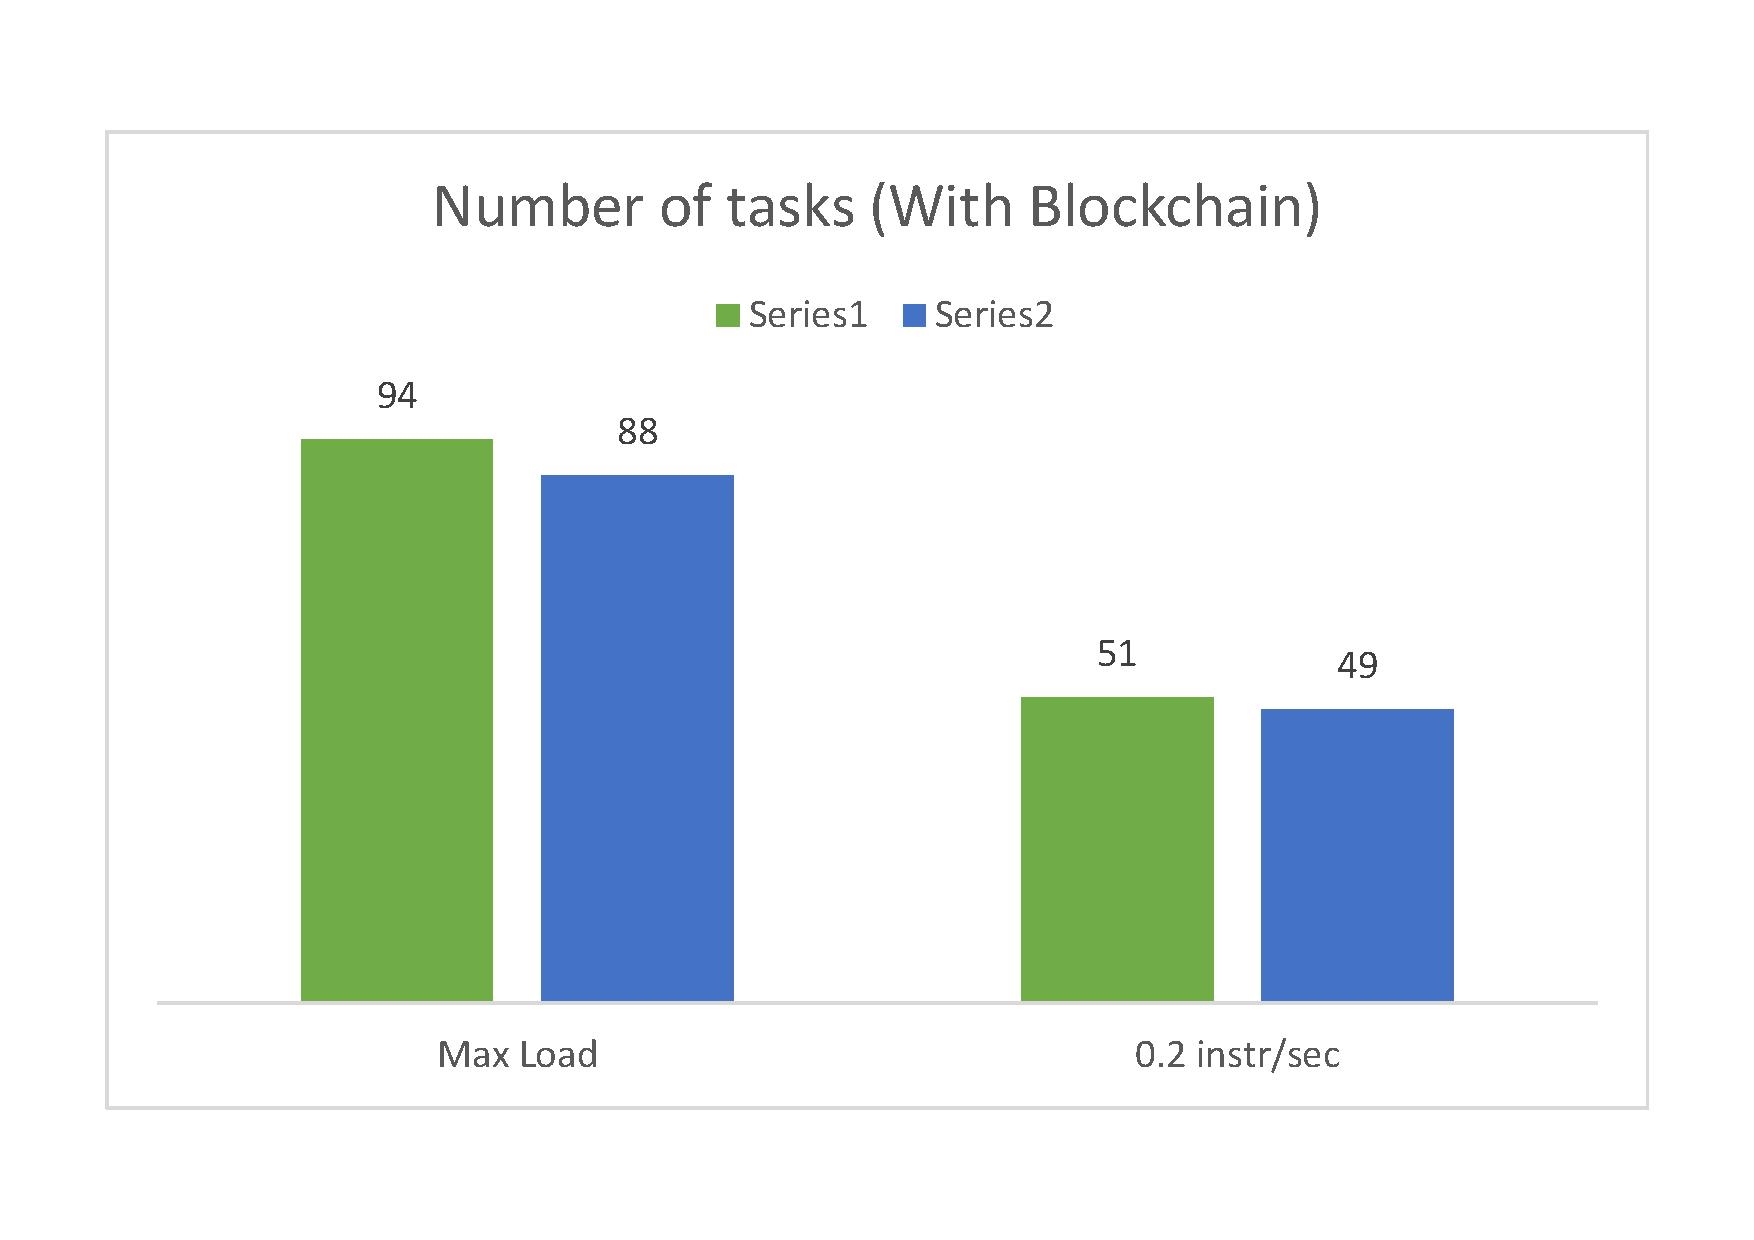
\includegraphics[width=6cm]{g11} \ \ \ \ \ \ \ \ \ \ \       
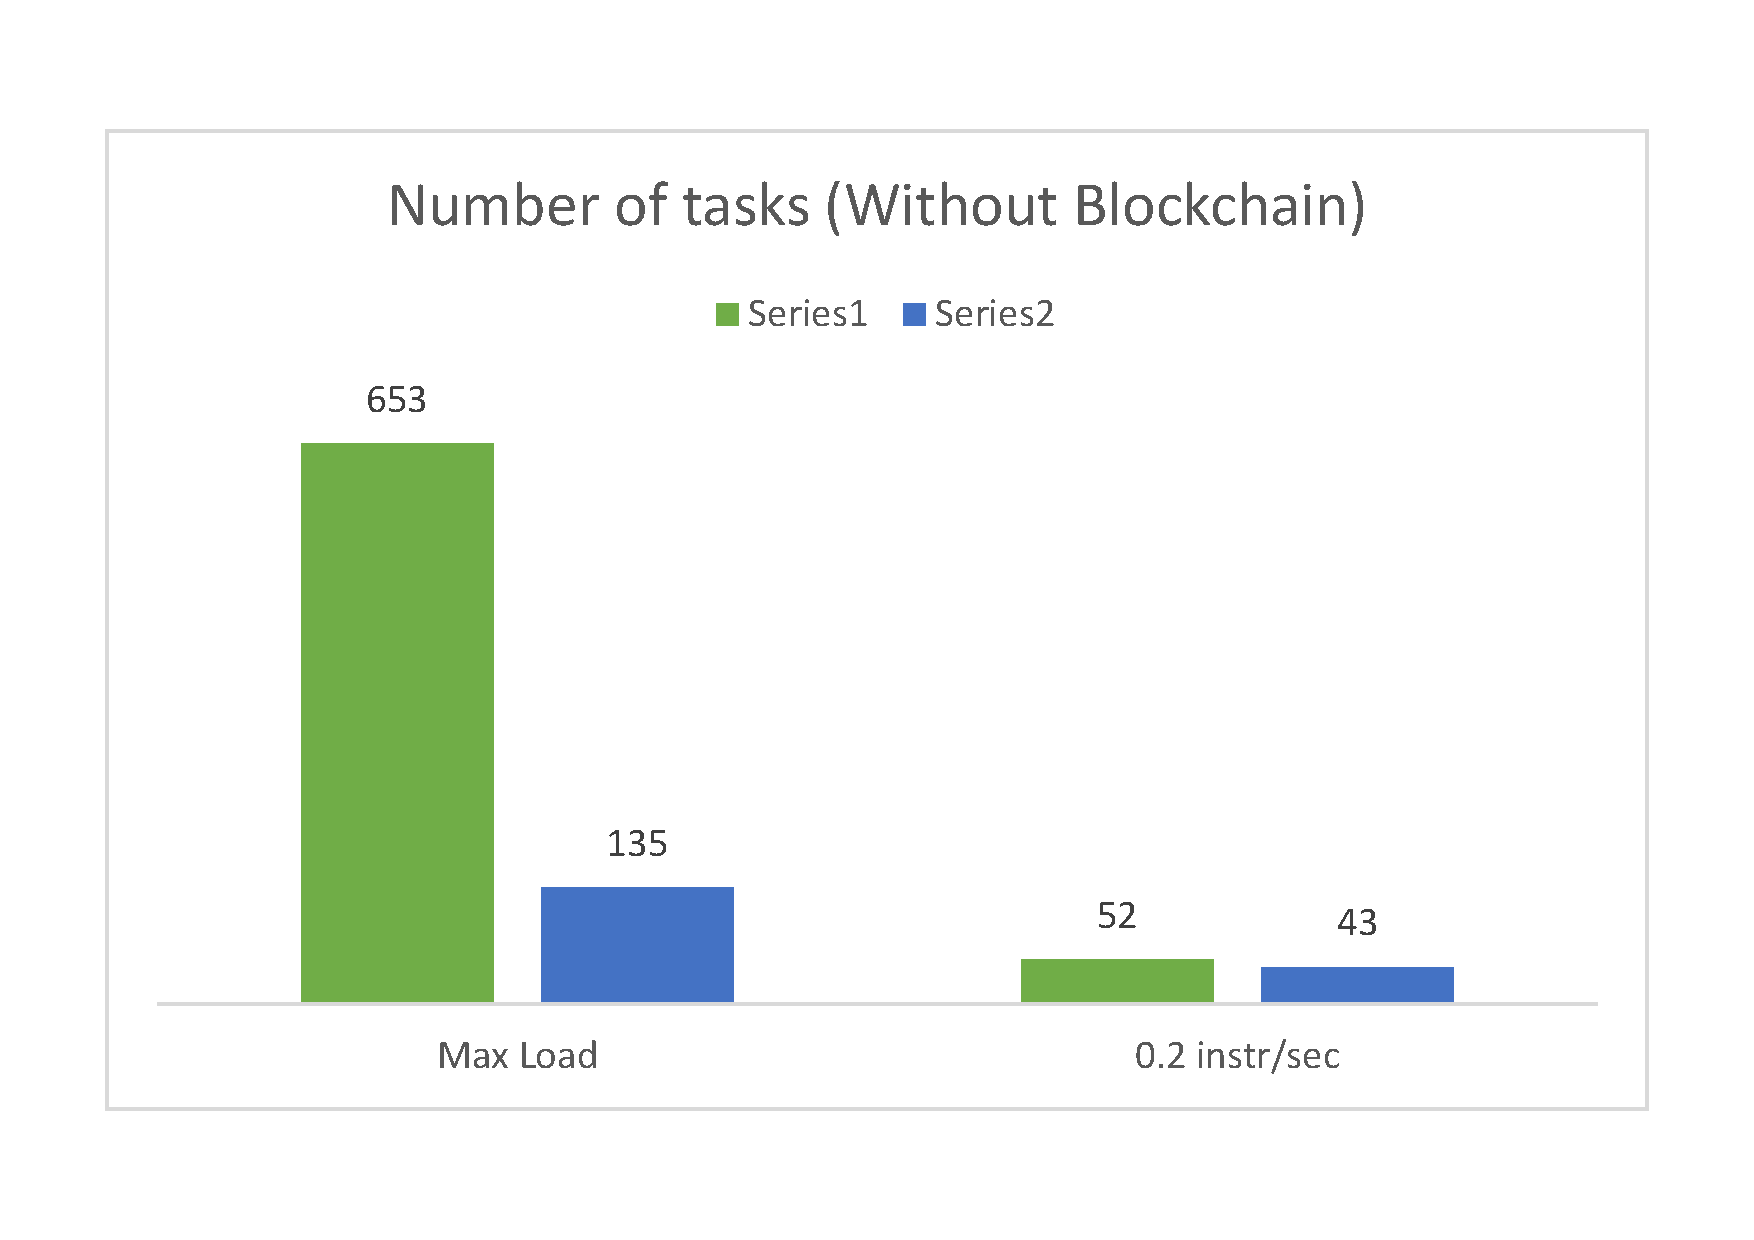
\includegraphics[width=6cm]{g12}
\captionof{figure}{Number of tasks performed in 5 minutes}
\end{figure}


\subsection{Latency}

Latency is another critical parameter for mission critical applications like healthcare, robotics, etc. Latency is inversely proportional to the Number of tasks. The results show that the latency in Fog case is much lesser than the Cloud Only case. Also similar to the previous parameter, without blockchain the latency is lower due to signature verification and proof of work validation that needs to be done with blockchain. Results show that computing in the Fog Only case not only cuts down response time but also safeguards the application from scalability issues (leading to delayed responses) arising due to large topologies and high data-generation rates.
\begin{figure}[h]
\centering
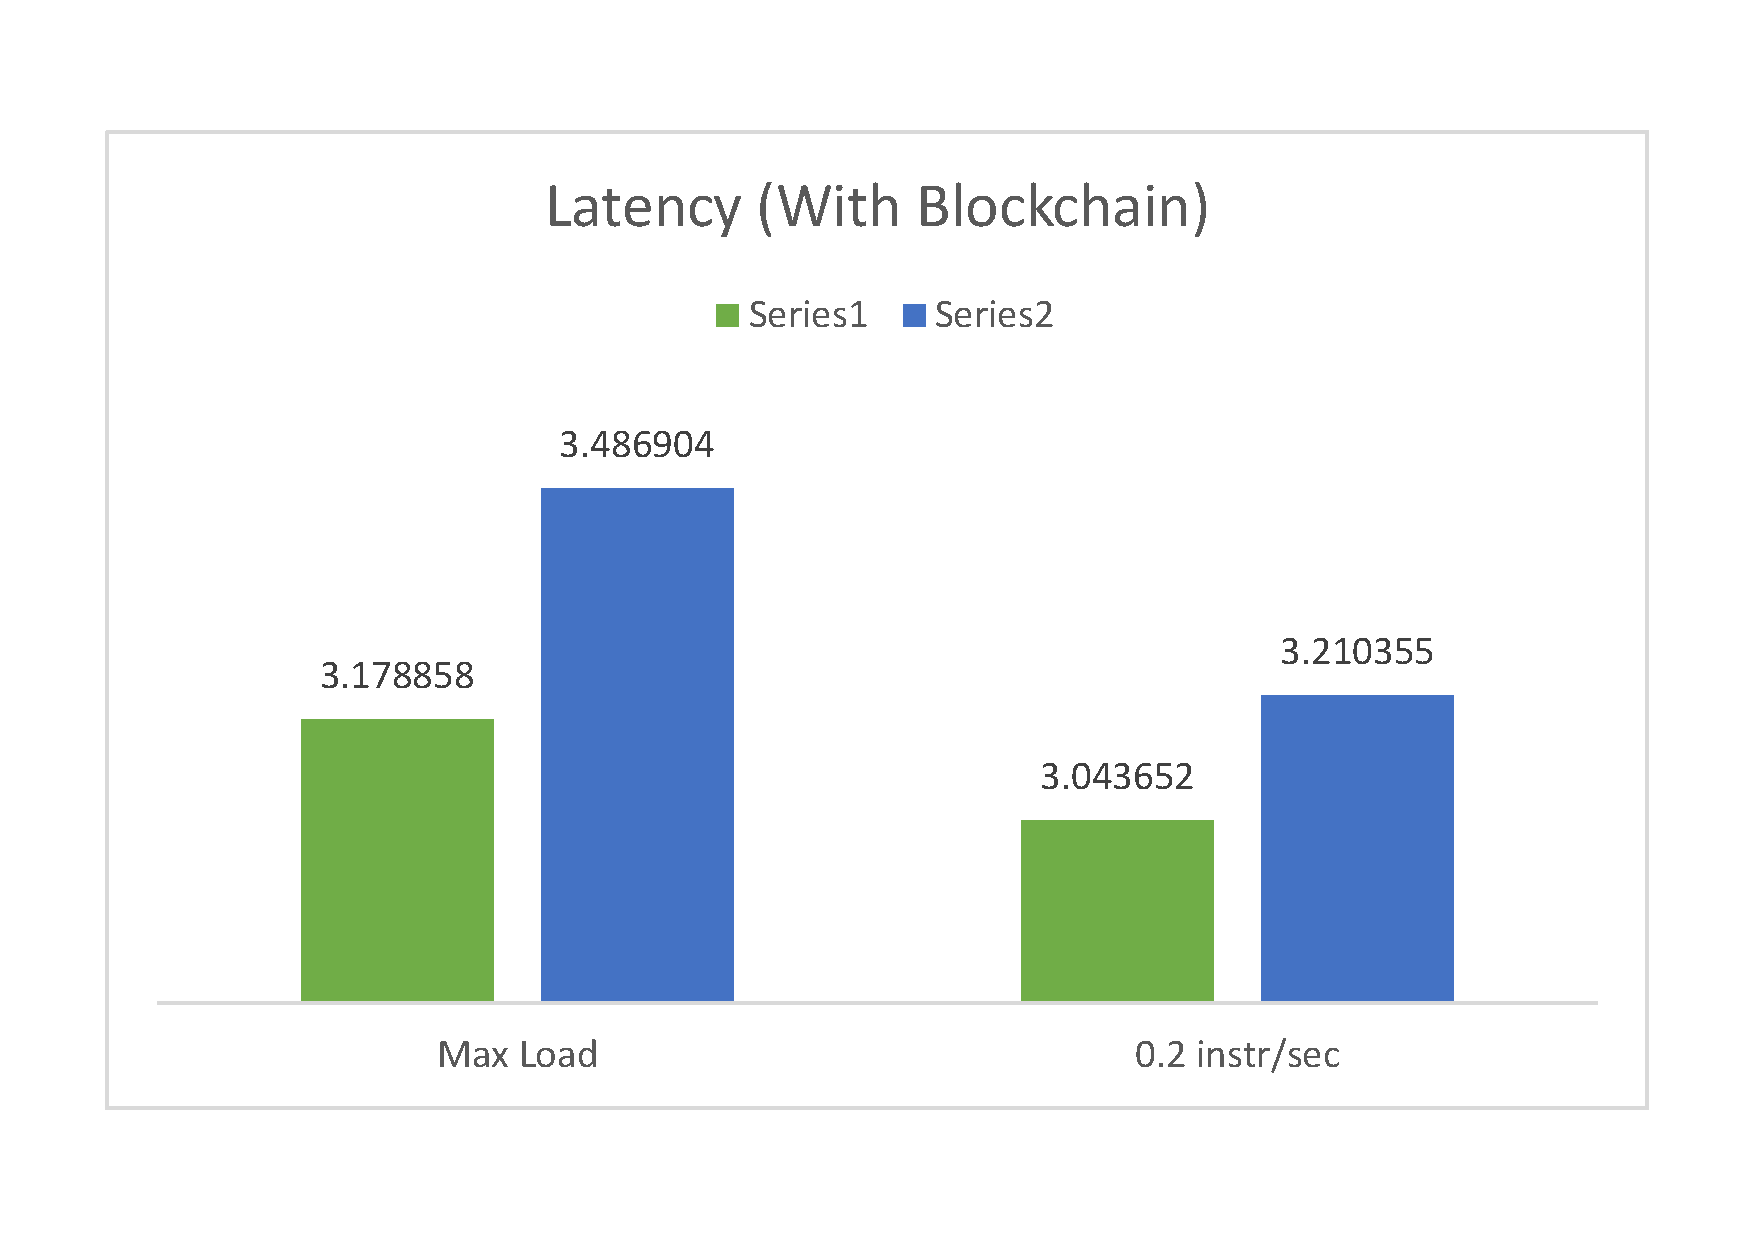
\includegraphics[width=6cm]{g71} \ \ \ \ \ \ \ \ \ \ \       
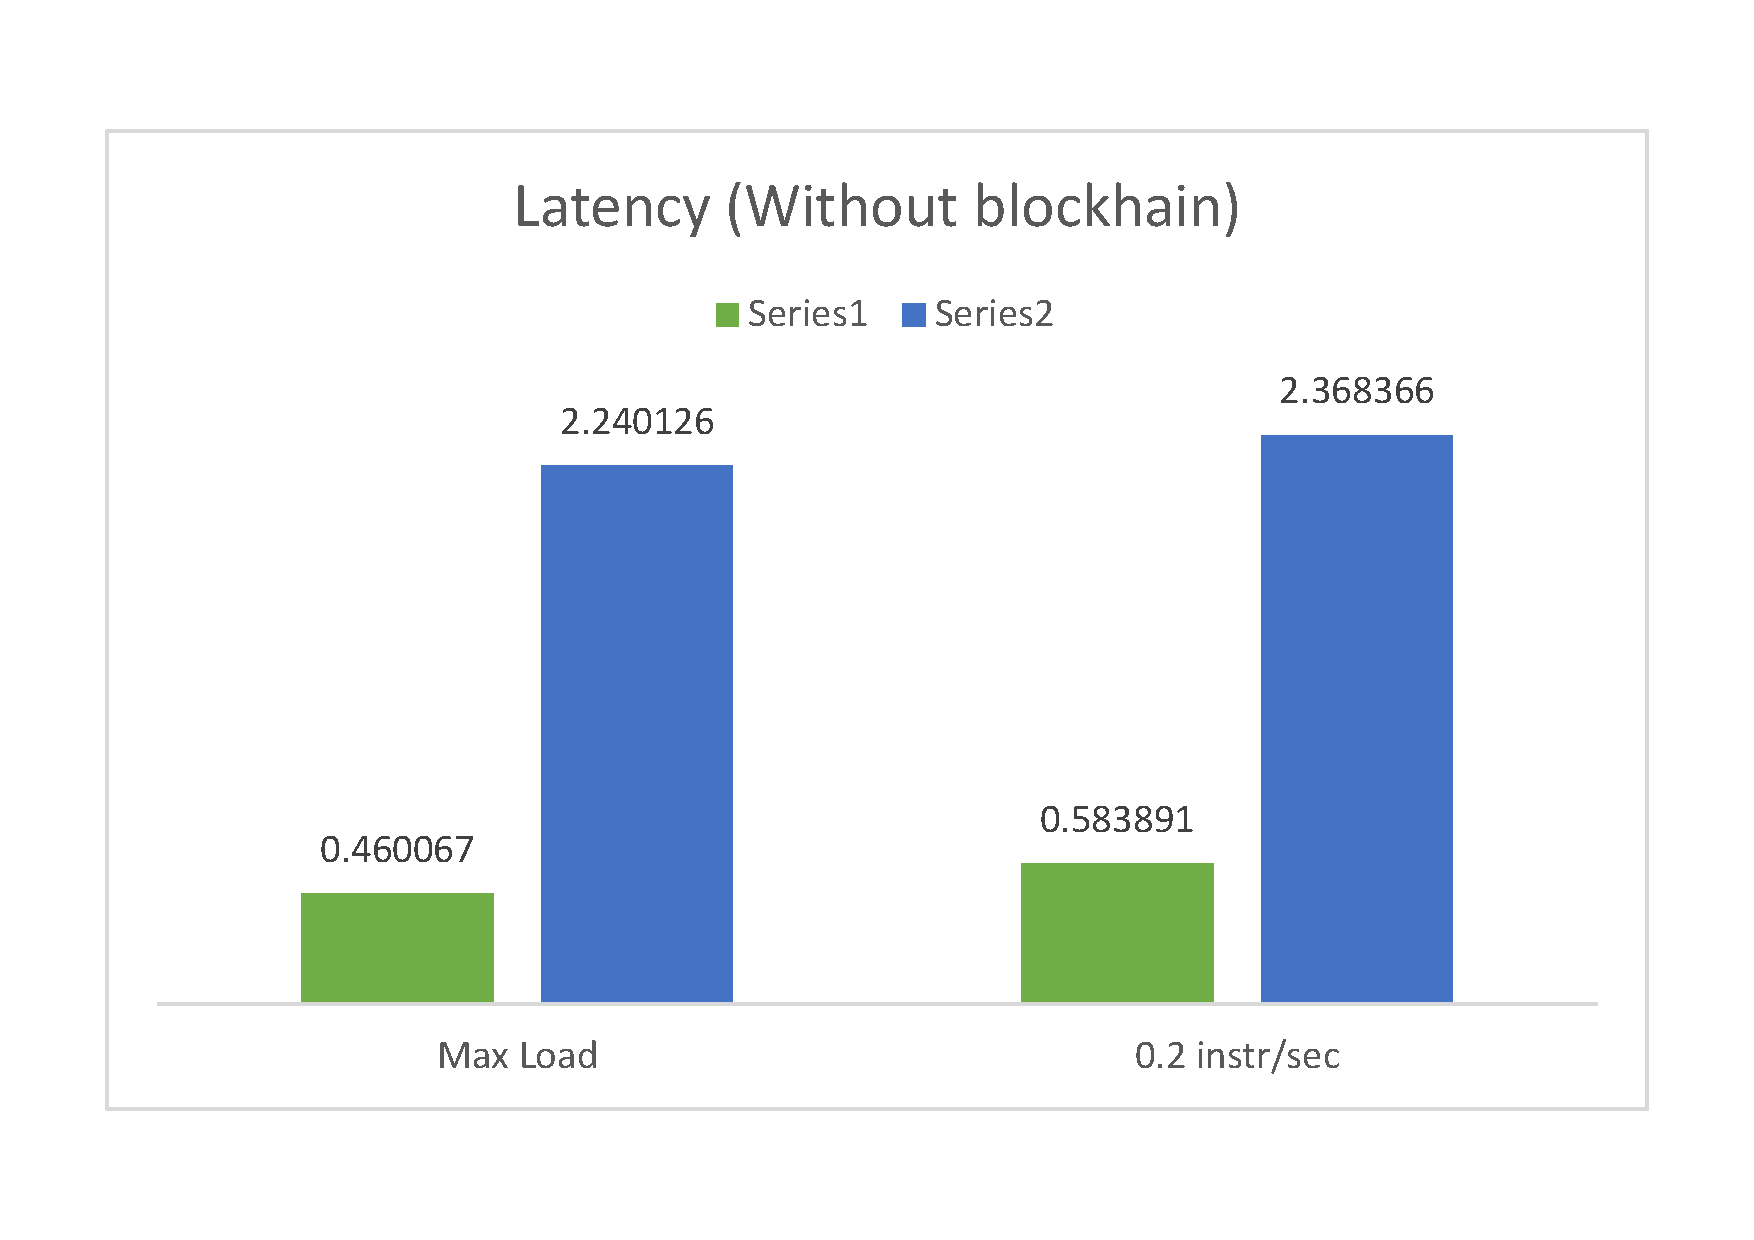
\includegraphics[width=6cm]{g72}
\captionof{figure}{Latency}
\end{figure}

\subsection{Network Usage}

Network usage is a significant factor in such systems. It is not only important for the Network Bandwidth requirements but also the data I/O capabilities of devices. If the Network Router can not support the required I/O of the framework then it can lead to network congestion and even breakdown of the full system. Thus it is important for the framework to balance Network usage and keep is as low as possible. Network Usage is calculated as: $(Number\ of\ bytes\ sent\ /\ second\ +\ Number\ of\ bytes\ received\ /\ second)/(Number\ of\ tasks)$, where bytes sent or received are by master node. Network Usage is lower in the Fog Only case as Aneka overhead of Network communication is not present in this situation. Also, without blockchain a lot of data sharing is eliminated which is there in the blockchain case for signature verification, blockchain hash data, public keys, etc.
\begin{figure}[h]
\centering
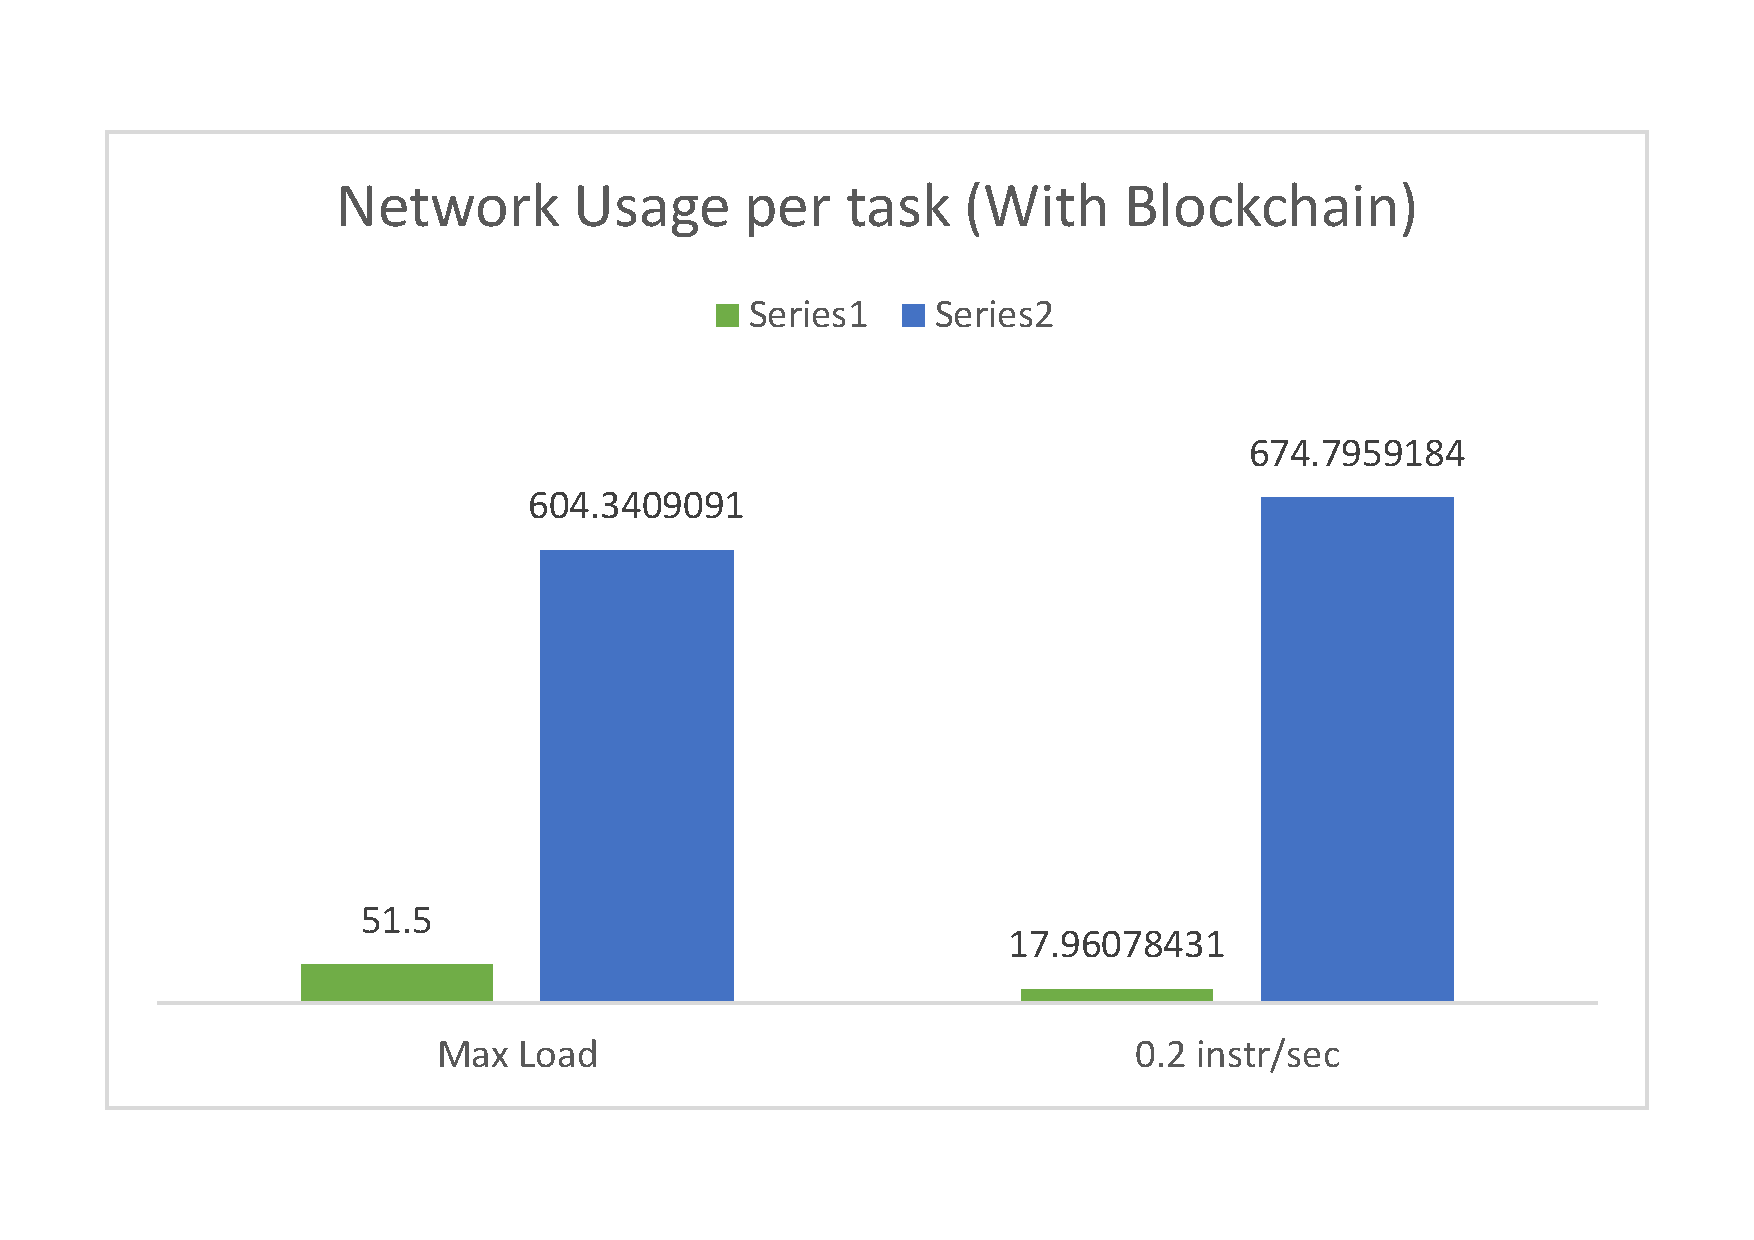
\includegraphics[width=6cm]{g61} \ \ \ \ \ \ \ \ \ \ \       
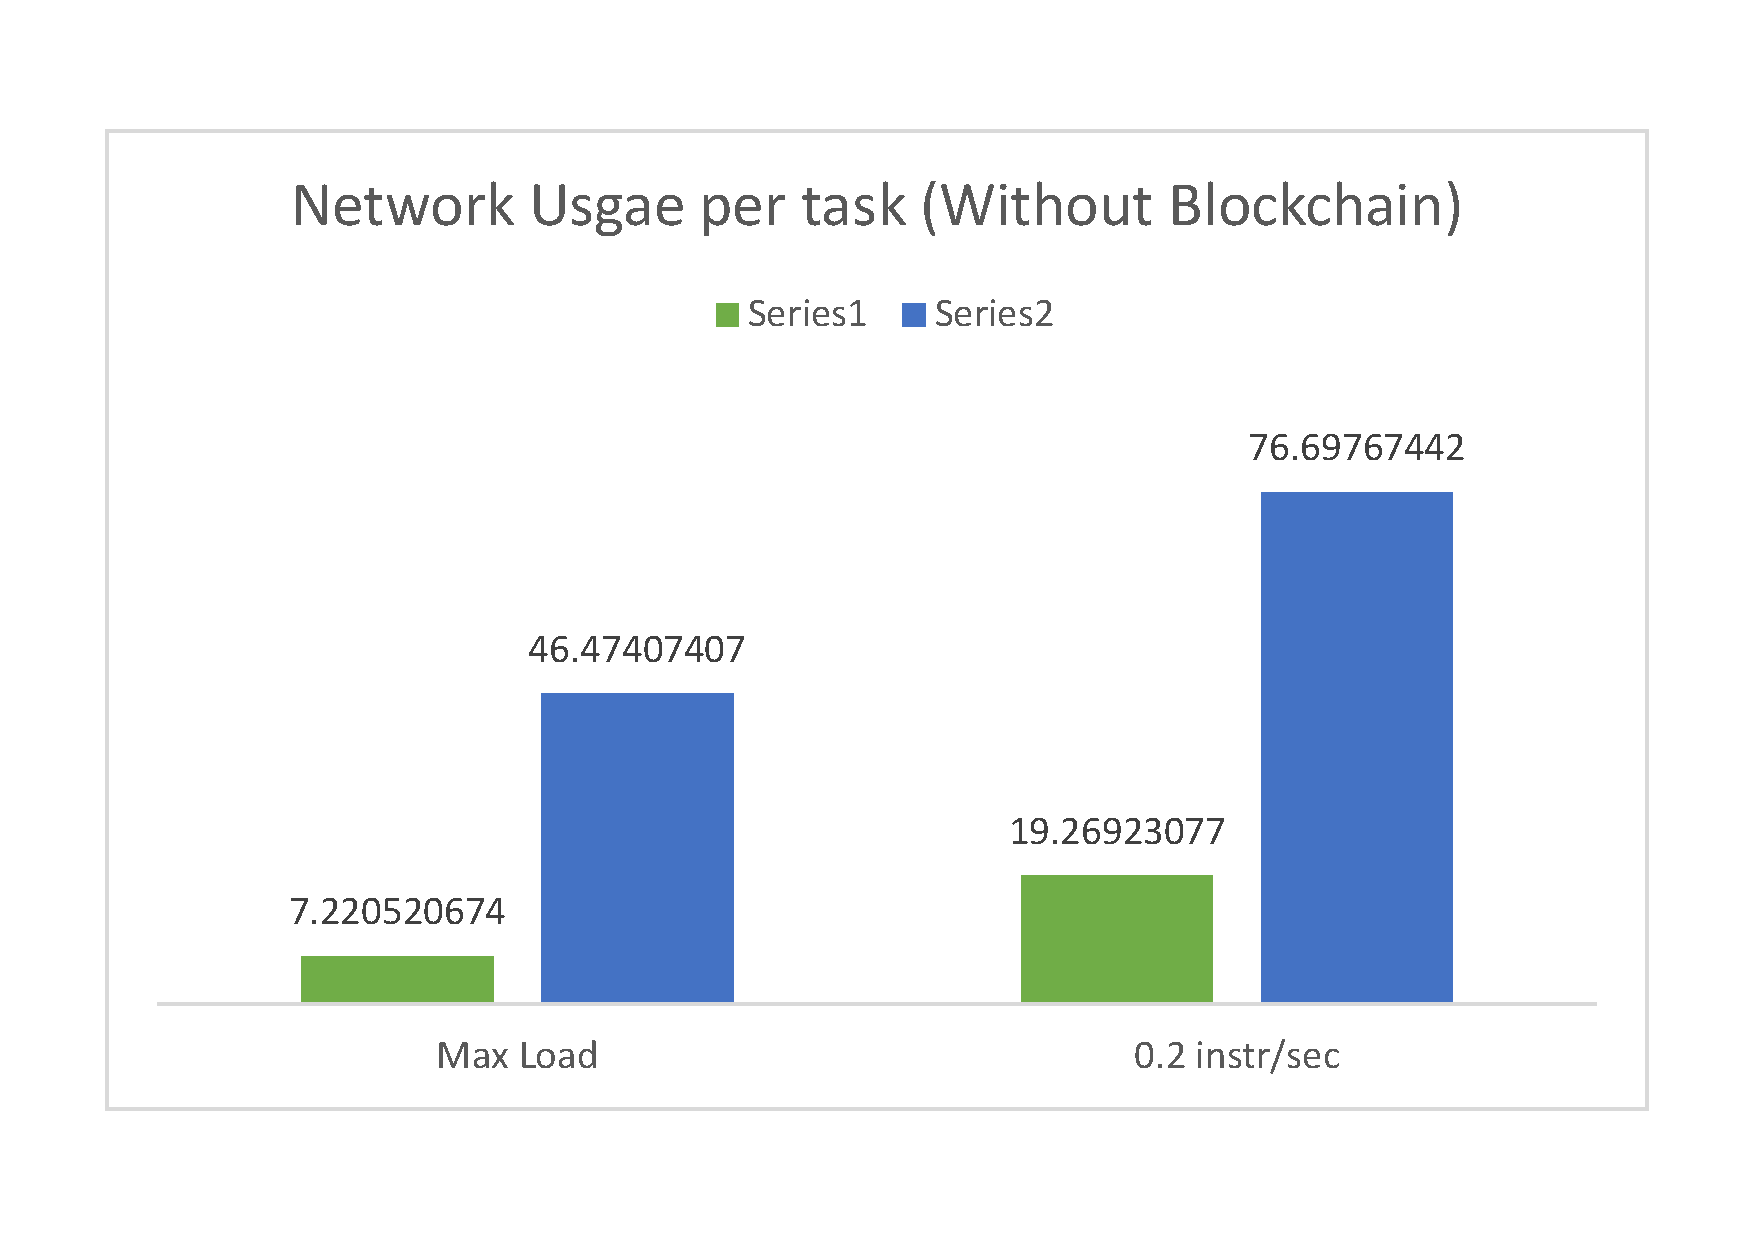
\includegraphics[width=6cm]{g62}
\captionof{figure}{Network Usage}
\end{figure}

\subsection{Energy}

Energy consumption is a very important parameter for deploying such network of computing devices. After the installation cost, the Energy consumption plays an important role in the maintenance costs of the system. In these tests the Energy coonsumption per task was calculated as $(Average\ Power\ Consumption\ \times\ 300\ seconds)/(Number\ of\ tasks)$. Energy consumption is also lower in the Fog case which is because the cloud power consumption is much higher as compared to edge devices. Average power consumption of a Raspberry Pi is 1.5W and that of a Windows Machine is 115W which is around 77 times the former. This makes maintenance of Fog devices much easier due to low expenditure on energy consumed. 
\begin{figure}[h]
\centering
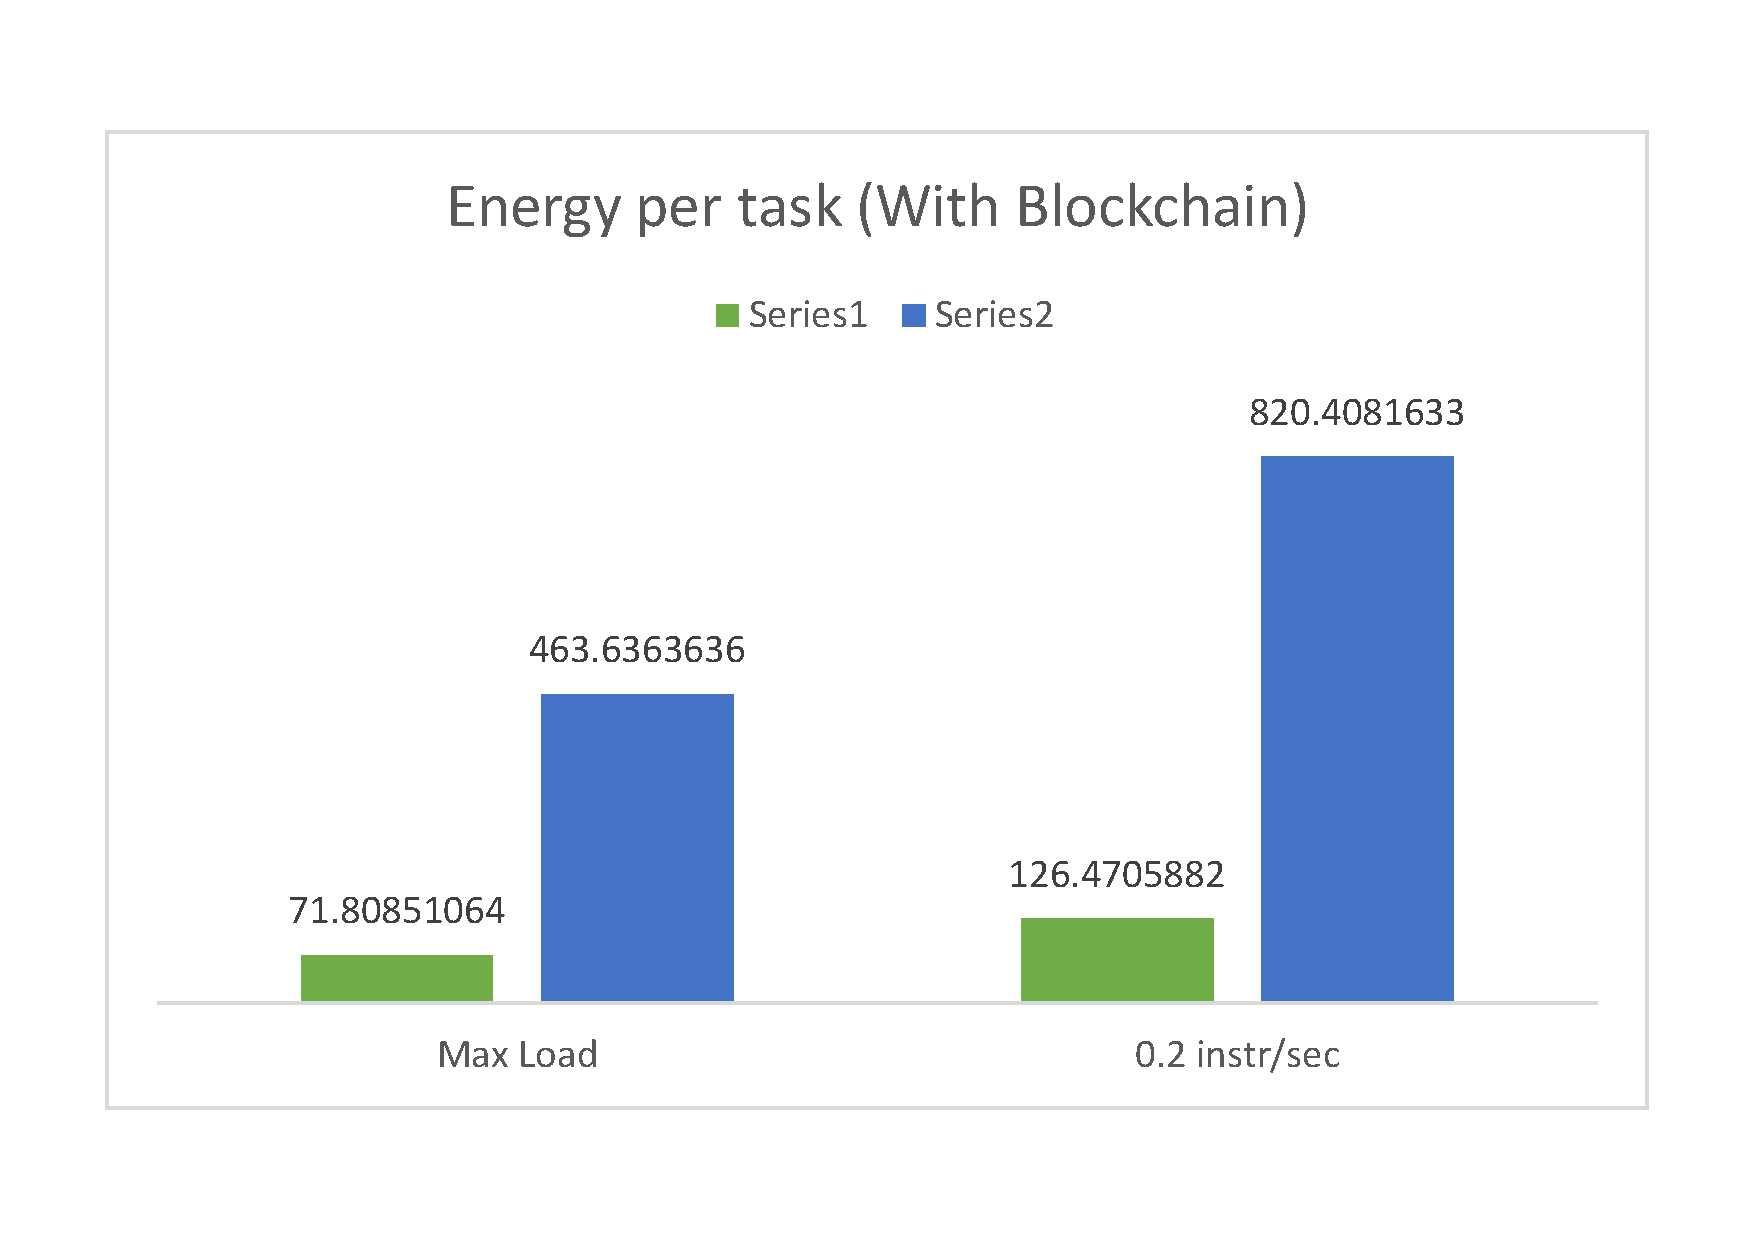
\includegraphics[width=6cm]{g31} \ \ \ \ \ \ \ \ \ \ \       
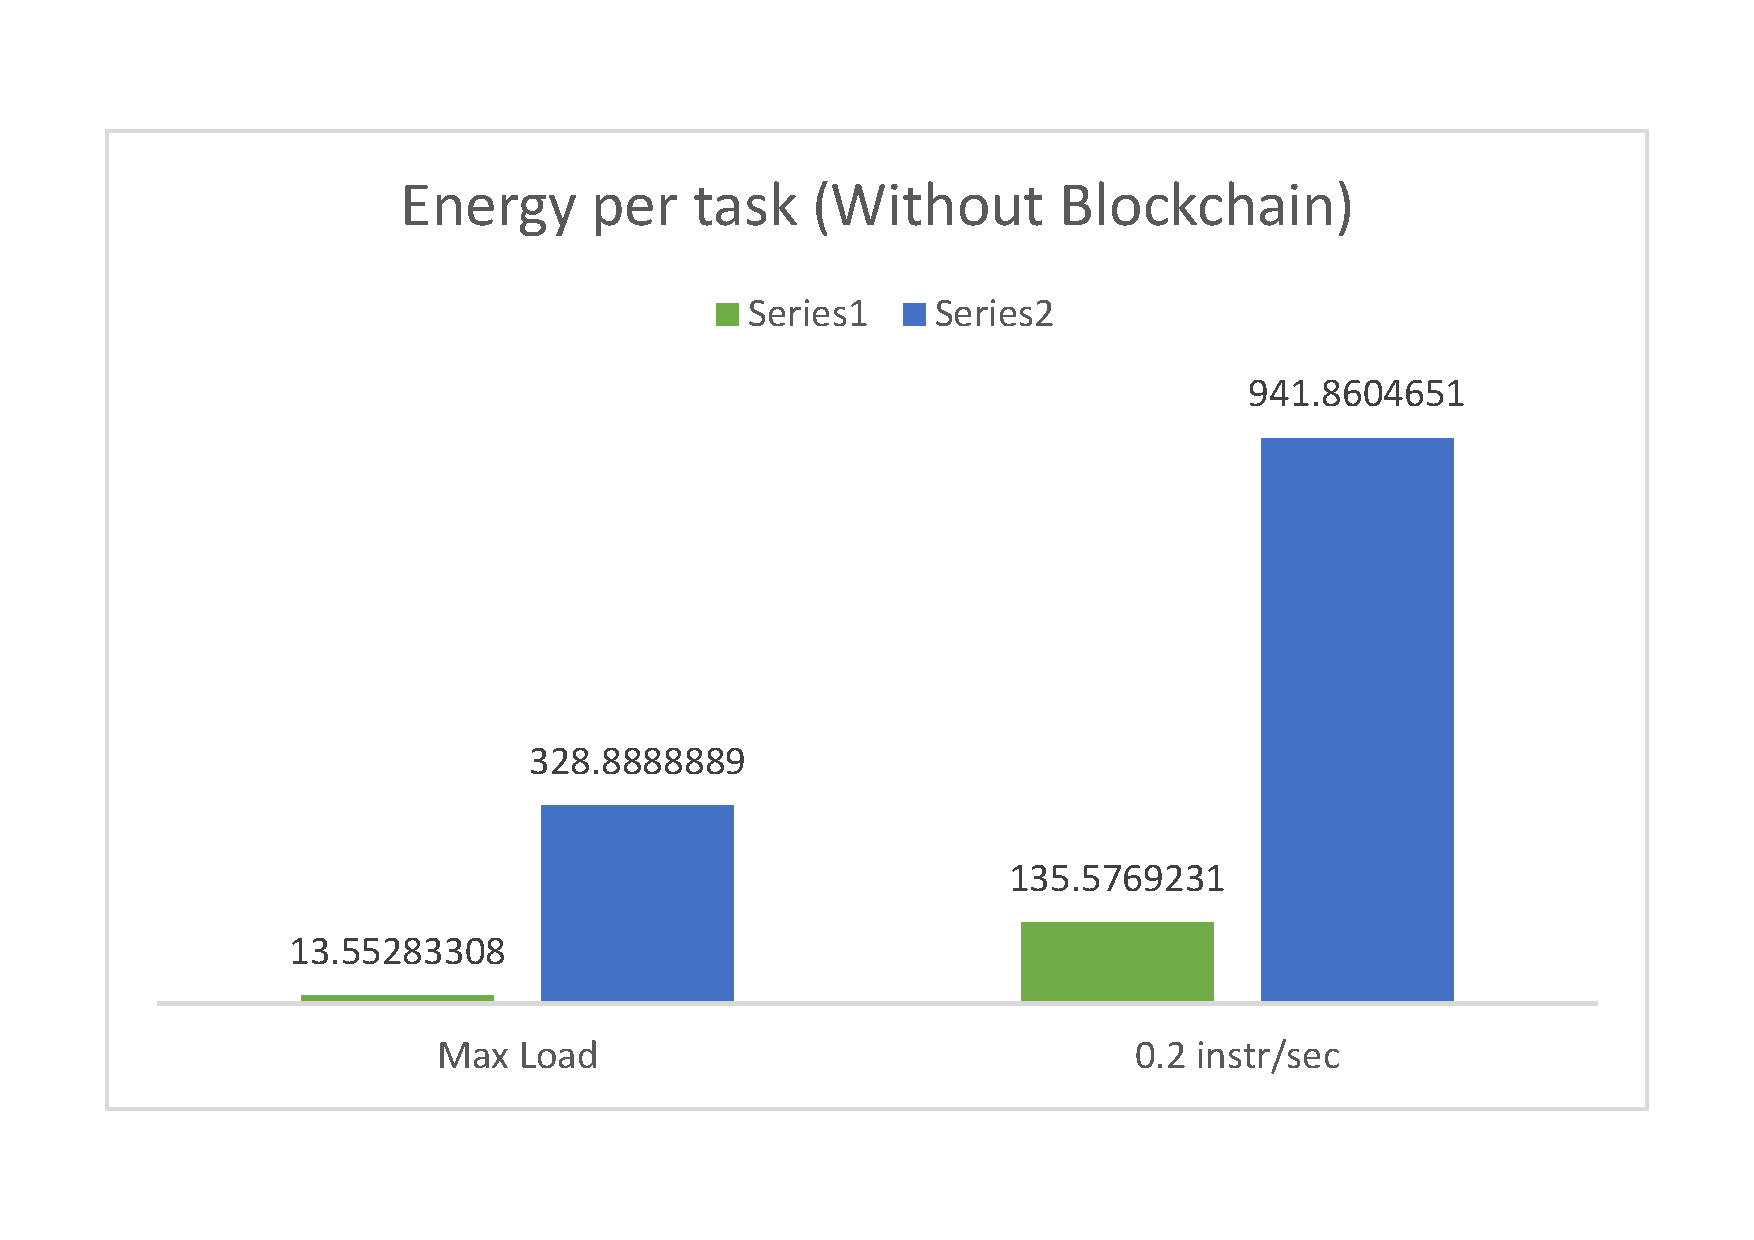
\includegraphics[width=6cm]{g32}
\captionof{figure}{Energy Used per task}
\end{figure}

\subsection{Master Node CPU, RAM, Cache Usage}

The Figure 12 shows the Master CPU, RAM and Cache usage for the Master node for each case. Series1: Fog Only without blockchain, Series2: Cloud Only without blockchain, Series3: Fog Only with blockchain, and Series4: Cloud Only with blockchain. The parameter values are much lower in the Fog Only case due to elimination of Aneka overhead. Even without blockchain these parameters are lower due to elimination of hash creation, mining, etc tasks.
\begin{figure}[h]
\centering
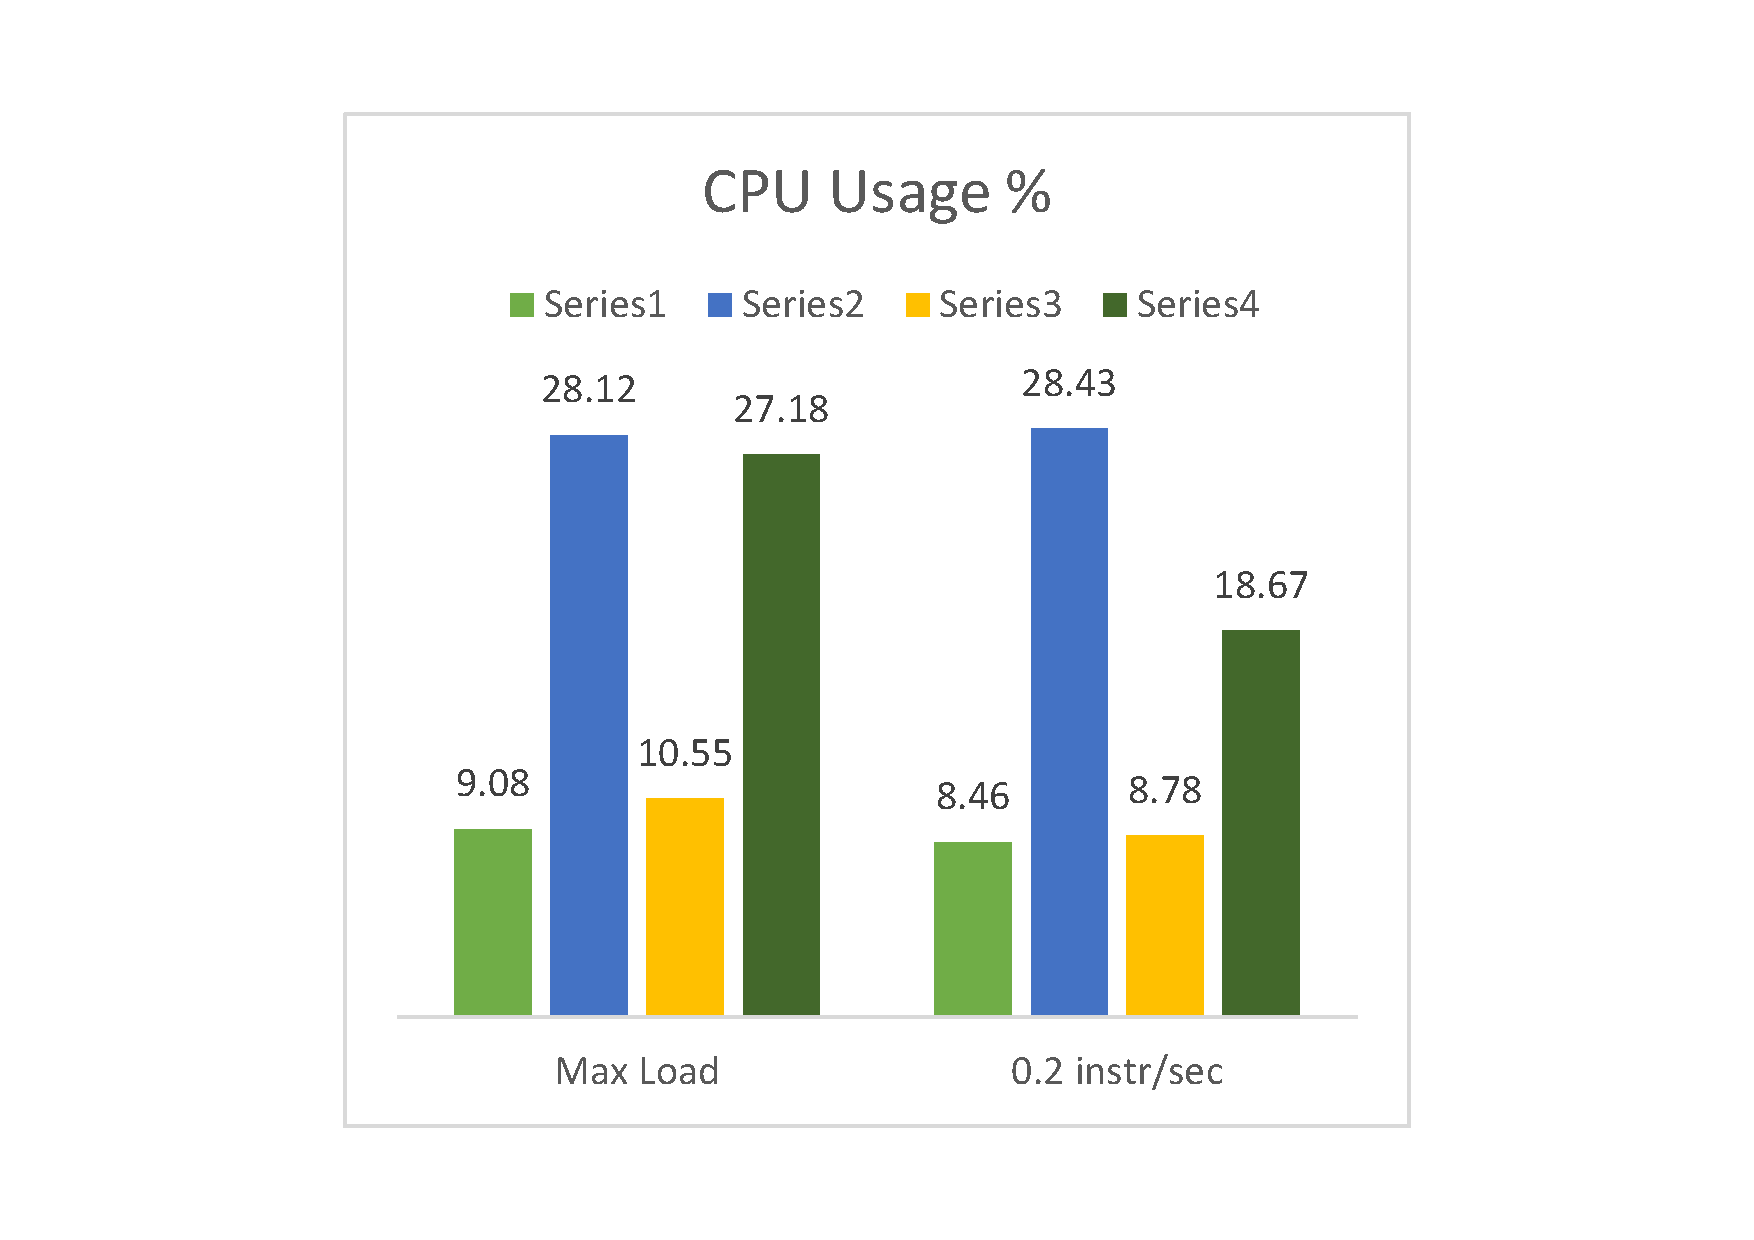
\includegraphics[width=5.5cm]{g81} \ \  
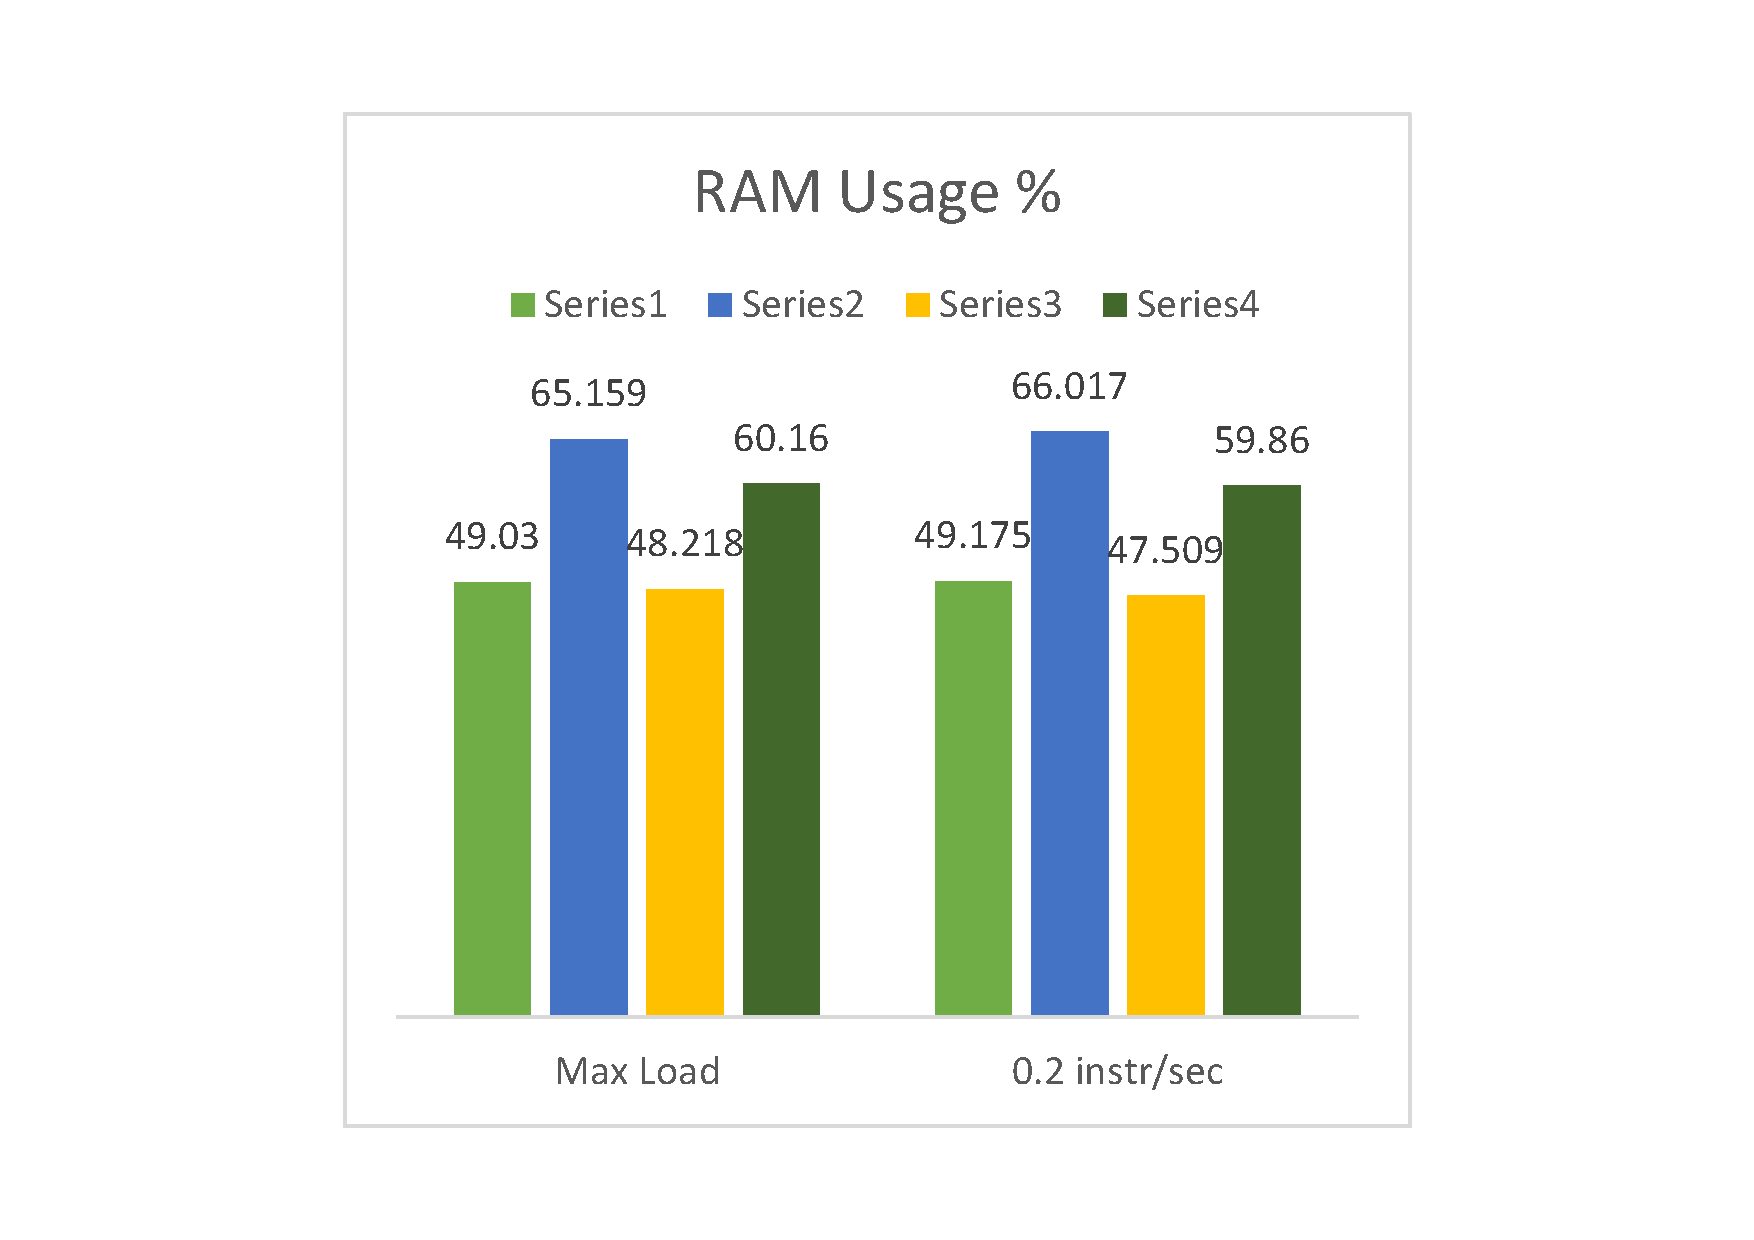
\includegraphics[width=5.5cm]{g82} \ \ 
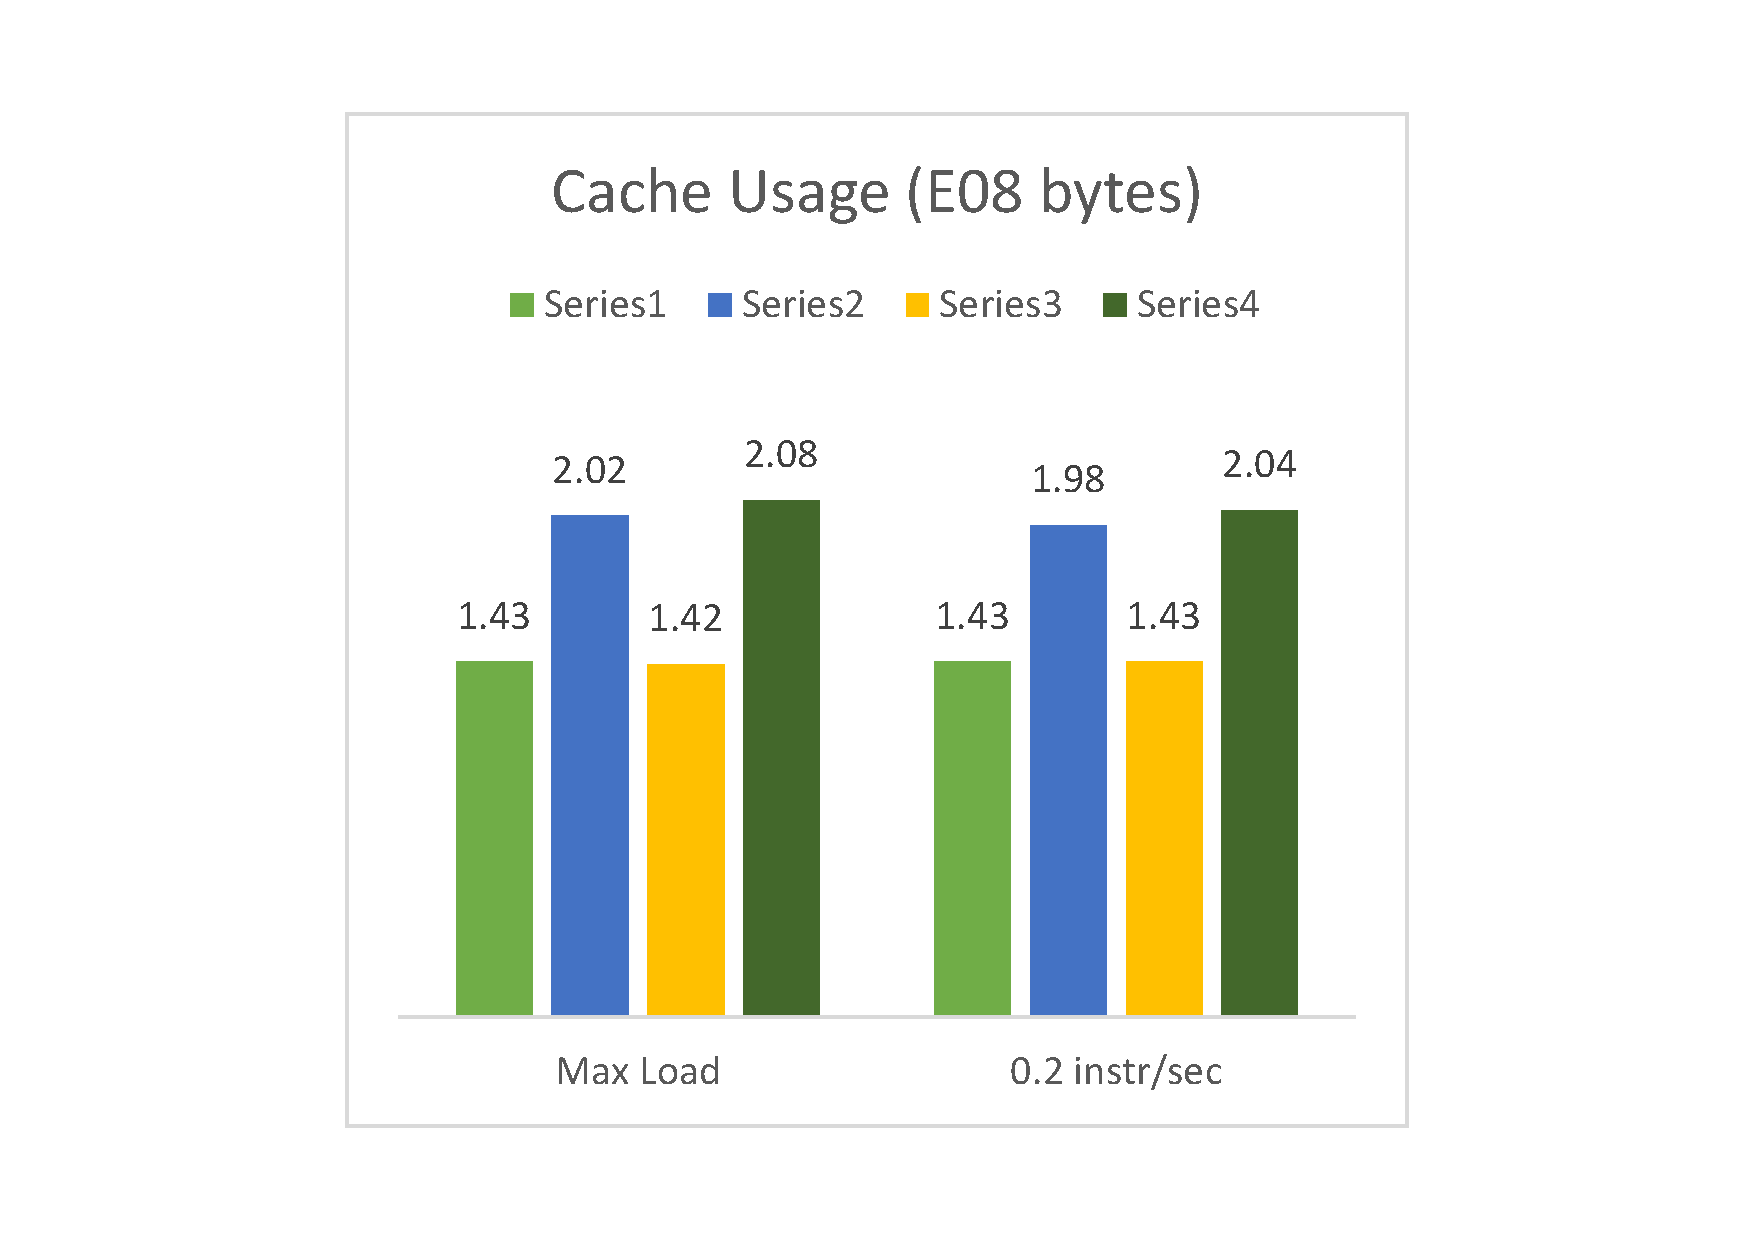
\includegraphics[width=5.5cm]{g83}
\captionof{figure}{Master CPU Usage \%}
\end{figure}

\subsection{Discussion}

From the results it is clear that Without blockchain case is much better in terms of latency, Network Usage, CPU Usage, etc. This is because of the much lesser load on the nodes for sharing data and maintaining blockchains.\\ 
We see that for the Sleep Apnea analysis case study, the Fog domain is much more favorable. Due to lesser latency, lower network usage, lesser energy consumption, etc. the Fog environment is much more suited for this type of applications. For application that involve high computation like calculating Fast Fourier Transform or involving Matrix Multiplication, the Fog devices may not be able to perform well in such calculation and the Cloud would be more suitable. Due to the light-weight computation requirement of Sleep Apnea Analysis application that we have deployed in our case study; the Fog domain is more suitable.

\section{Future Work}
This software forms a base for setting up Fog Computing Environment which is not OS or architecture specific. Though the framework is complete by itself and fully functions to perform real-time, sensor-based Sleep Apnea analysis and can be used for other applications as well, but has a large scope of improvement and further developments:

\subsection{Load Balancing Scheme}
As discussed earlier, the current load balancing scheme is naive and can be greatly improved. Currently, the load balancing scheme focuses on task distribution based on CPU load, whichever device has the least load, the task is given to it. There can be a cumulative ranking parameter which takes into account many other factors as per requirement. These factors can be and are not limited to: Network Bandwidth, Memory Load, etc. Different weights can be given to these parameters are per the scenario. 

\subsection{Data Integrity}
Health Analysis data is important for patients as their treatment and lives depend on it, thus it is important to save this data from fraudulent manipulation or sabotage from hackers. Thus, to maintain data integrity many techniques like Blockchain can be implemented to ensure that data is secure. 

\subsection{Data Privacy}
Some applications require data to be secure as well as kept private. The current system is prone to attacks and unwanted display of data to others. Privacy policies like encrypting the data can be used to ensure that the data cannot be seen by others. 

\subsection{Data Authenticity}
The current system allows any device to connect to master and share or view data. This can be used by hackers to forge DDoS or similar attacks. As Fog platforms also contains low range devices with limited threshold management, such attacks even at a low scale can destroy such devices. Thus, a signature-based validation technique can be used to ensure user and data authenticity.


\section{Conclusions}

\section{Software Availability}





% An example of a floating figure using the graphicx package.
% Note that \label must occur AFTER (or within) \caption.
% For figures, \caption should occur after the \includegraphics.
% Note that IEEEtran v1.7 and later has special internal code that
% is designed to preserve the operation of \label within \caption
% even when the captionsoff option is in effect. However, because
% of issues like this, it may be the safest practice to put all your
% \label just after \caption rather than within \caption{}.
%
% Reminder: the "draftcls" or "draftclsnofoot", not "draft", class
% option should be used if it is desired that the figures are to be
% displayed while in draft mode.
%
%\begin{figure}[!t]
%\centering
%\includegraphics[width=2.5in]{myfigure}
% where an .eps filename suffix will be assumed under latex, 
% and a .pdf suffix will be assumed for pdflatex; or what has been declared
% via \DeclareGraphicsExtensions.
%\caption{Simulation results for the network.}
%\label{fig_sim}
%\end{figure}

% Note that the IEEE typically puts floats only at the top, even when this
% results in a large percentage of a column being occupied by floats.
% However, the Computer Society has been known to put floats at the bottom.


% An example of a double column floating figure using two subfigures.
% (The subfig.sty package must be loaded for this to work.)
% The subfigure \label commands are set within each subfloat command,
% and the \label for the overall figure must come after \caption.
% \hfil is used as a separator to get equal spacing.
% Watch out that the combined width of all the subfigures on a 
% line do not exceed the text width or a line break will occur.
%
%\begin{figure*}[!t]
%\centering
%\subfloat[Case I]{\includegraphics[width=2.5in]{box}%
%\label{fig_first_case}}
%\hfil
%\subfloat[Case II]{\includegraphics[width=2.5in]{box}%
%\label{fig_second_case}}
%\caption{Simulation results for the network.}
%\label{fig_sim}
%\end{figure*}
%
% Note that often IEEE papers with subfigures do not employ subfigure
% captions (using the optional argument to \subfloat[]), but instead will
% reference/describe all of them (a), (b), etc., within the main caption.
% Be aware that for subfig.sty to generate the (a), (b), etc., subfigure
% labels, the optional argument to \subfloat must be present. If a
% subcaption is not desired, just leave its contents blank,
% e.g., \subfloat[].


% An example of a floating table. Note that, for IEEE style tables, the
% \caption command should come BEFORE the table and, given that table
% captions serve much like titles, are usually capitalized except for words
% such as a, an, and, as, at, but, by, for, in, nor, of, on, or, the, to
% and up, which are usually not capitalized unless they are the first or
% last word of the caption. Table text will default to \footnotesize as
% the IEEE normally uses this smaller font for tables.
% The \label must come after \caption as always.
%
%\begin{table}[!t]
%% increase table row spacing, adjust to taste
%\renewcommand{\arraystretch}{1.3}
% if using array.sty, it might be a good idea to tweak the value of
% \extrarowheight as needed to properly center the text within the cells
%\caption{An Example of a Table}
%\label{table_example}
%\centering
%% Some packages, such as MDW tools, offer better commands for making tables
%% than the plain LaTeX2e tabular which is used here.
%\begin{tabular}{|c||c|}
%\hline
%One & Two\\
%\hline
%Three & Four\\
%\hline
%\end{tabular}
%\end{table}


% Note that the IEEE does not put floats in the very first column
% - or typically anywhere on the first page for that matter. Also,
% in-text middle ("here") positioning is typically not used, but it
% is allowed and encouraged for Computer Society conferences (but
% not Computer Society journals). Most IEEE journals/conferences use
% top floats exclusively. 
% Note that, LaTeX2e, unlike IEEE journals/conferences, places
% footnotes above bottom floats. This can be corrected via the
% \fnbelowfloat command of the stfloats package.




\section{Conclusion}
The conclusion goes here.





% if have a single appendix:
%\appendix[Proof of the Zonklar Equations]
% or
%\appendix  % for no appendix heading
% do not use \section anymore after \appendix, only \section*
% is possibly needed

% use appendices with more than one appendix
% then use \section to start each appendix
% you must declare a \section before using any
% \subsection or using \label (\appendices by itself
% starts a section numbered zero.)
%


\appendices

% use section* for acknowledgment
\ifCLASSOPTIONcompsoc
  % The Computer Society usually uses the plural form
  \section*{Acknowledgments}
\else
  % regular IEEE prefers the singular form
  \section*{Acknowledgment}
\fi


The authors would like to thank...


% Can use something like this to put references on a page
% by themselves when using endfloat and the captionsoff option.
\ifCLASSOPTIONcaptionsoff
  \newpage
\fi



% trigger a \newpage just before the given reference
% number - used to balance the columns on the last page
% adjust value as needed - may need to be readjusted if
% the document is modified later
%\IEEEtriggeratref{8}
% The "triggered" command can be changed if desired:
%\IEEEtriggercmd{\enlargethispage{-5in}}

% references section

% can use a bibliography generated by BibTeX as a .bbl file
% BibTeX documentation can be easily obtained at:
% http://mirror.ctan.org/biblio/bibtex/contrib/doc/
% The IEEEtran BibTeX style support page is at:
% http://www.michaelshell.org/tex/ieeetran/bibtex/
%\bibliographystyle{IEEEtran}
% argument is your BibTeX string definitions and bibliography database(s)
%\bibliography{IEEEabrv,../bib/paper}
%
% <OR> manually copy in the resultant .bbl file
% set second argument of \begin to the number of references
% (used to reserve space for the reference number labels box)
\begin{thebibliography}{1}

\bibitem{IEEEhowto:kopka}
H.~Kopka and P.~W. Daly, \emph{A Guide to \LaTeX}, 3rd~ed.\hskip 1em plus
  0.5em minus 0.4em\relax Harlow, England: Addison-Wesley, 1999.

\end{thebibliography}

% biography section
% 
% If you have an EPS/PDF photo (graphicx package needed) extra braces are
% needed around the contents of the optional argument to biography to prevent
% the LaTeX parser from getting confused when it sees the complicated
% \includegraphics command within an optional argument. (You could create
% your own custom macro containing the \includegraphics command to make things
% simpler here.)
%\begin{IEEEbiography}[{\includegraphics[width=1in,height=1.25in,clip,keepaspectratio]{mshell}}]{Michael Shell}
% or if you just want to reserve a space for a photo:

\begin{IEEEbiography}{Shreshth Tuli}
Biography text here.
\end{IEEEbiography}

% if you will not have a photo at all:
\begin{IEEEbiographynophoto}{Shikhar Tuli}
Biography text here.
\end{IEEEbiographynophoto}

% insert where needed to balance the two columns on the last page with
% biographies
%\newpage

\begin{IEEEbiographynophoto}{Redowan Mahmud}
Biography text here.
\end{IEEEbiographynophoto}

% You can push biographies down or up by placing
% a \vfill before or after them. The appropriate
% use of \vfill depends on what kind of text is
% on the last page and whether or not the columns
% are being equalized.

%\vfill

% Can be used to pull up biographies so that the bottom of the last one
% is flush with the other column.
%\enlargethispage{-5in}



% that's all folks
\end{document}


